\documentclass{report}


\usepackage{amsmath} % Better matrix environment
\usepackage{amssymb}
% \usepackage{enumitem}
\usepackage{etoolbox} % If conditions
\usepackage{graphicx}
\usepackage{listings} % for code
\usepackage{paralist} % inline numbering
\usepackage{caption}
\usepackage{subcaption}
\usepackage{tikz}
\usepackage{tikz-qtree,tikz-qtree-compat} % Trees
\usepackage{xkeyval}


% Squiggly lines
\usetikzlibrary{decorations.pathmorphing}


% Node shapes
\usetikzlibrary{shapes,decorations}

\newcommand{\VertexSet}{V}
\newcommand{\CellSet}{C}

\newcommand{\Visited}{V_{visited}}

% Adjacency relation
\newcommand{\AdjVV}{Adj_{\VertexSet\VertexSet}}

% Cardinality of
\newcommand{\card}[1]{\left\vert{#1}\right\vert}

% powerset of
\newcommand{\powerset}[1]{\mathcal P \left({#1}\right)}


% Tikz function: compute absolute position
% row, delta-sy, y-offset
\newcommand{\rctoxy}[3][3=0]{#1*#2 + #3}



% Line that can go anywhere, structured region or outside
\tikzset{%
    anywhere/.style={
		decorate,
		decoration={
		    snake,
		    segment length=4,
		    amplitude=.9,post=lineto,
		    post length=2pt
		}
	}
}

% Line that can only go outside the structured region
\tikzset{outside/.style={dotted}}


% Ellipsis
\tikzset{ellipsis/.style={loosely dotted}}

% Structured
\tikzset{structured/.style={}}


%% Node labelling functions

% row, col, rowoffset, coloffset
\newcommand{\plainlabelnode}[4]{
\pgfmathtruncatemacro{\rowlabel}{#1+#3}\pgfmathtruncatemacro{\collabel}{#2+#4}$n_{\rowlabel,\collabel}$}

% row, col, rowoffset, coloffset, column-variable
\newcommand{\varcollabelnode}[5]{
\pgfmathtruncatemacro{\row}{#1+#3}\pgfmathtruncatemacro{\col}{#2+#4}\pgfmathtruncatemacro{\colzero}{\col-1}\newcommand{\collabel}{\ifnumcomp{\colzero}{=}{0}{#5}{\ifnumcomp{\colzero}{>}{0}{#5+\colzero}{#5\colzero}}}$n_{\row,\collabel}$}

% row, col, rowoffset, coloffset, row-variable
\newcommand{\varrowlabelnode}[5]{\pgfmathtruncatemacro{\row}{#1+#3}\pgfmathtruncatemacro{\rowzero}{\row-1}\pgfmathtruncatemacro{\col}{#2+#4}\newcommand{\rowlabel}{\ifnumcomp{\rowzero}{=}{0}{#5}{\ifnumcomp{\rowzero}{>}{0}{#5+\rowzero}{#5\rowzero}}}$n_{\rowlabel,\col}$}


% row, col, rowoffset, coloffset, row-variable, col-variable
\newcommand{\varlabelnode}[6]{\pgfmathtruncatemacro{\row}{#1+#3}\pgfmathtruncatemacro{\rowzero}{\row-1}\pgfmathtruncatemacro{\col}{#2+#4}\pgfmathtruncatemacro{\colzero}{\col-1}\newcommand{\rowlabel}{\ifnumcomp{\rowzero}{=}{0}{#5}{\ifnumcomp{\rowzero}{>}{0}{#5+\rowzero}{#5\rowzero}}}\newcommand{\collabel}{\ifnumcomp{\colzero}{=}{0}{#6}{\ifnumcomp{\colzero}{>}{0}{#6+\colzero}{#6\colzero}}}$n_{\rowlabel,\collabel}$}



\pgfkeys{/tikz/.cd,% to set the path
  rows/.get=\krows,
  rows/.store in=\krows,
  cols/.get=\kcols,
  cols/.store in=\kcols,
  rowoffset/.initial=0,
  rowoffset/.get=\krowoffset,
  rowoffset/.store in=\krowoffset,
  coloffset/.initial=0,
  coloffset/.get=\kcoloffset,
  coloffset/.store in=\kcoloffset,
  labeler/.get=\klabeler,
  labeler/.store in=\klabeler,
  labelerA/.get=\klabelerA,
  labelerA/.store in=\klabelerA,
  labelerB/.get=\klabelerB,
  labelerB/.store in=\klabelerB,
  labelerC/.get=\klabelerC,
  labelerC/.store in=\klabelerC,
  labelerD/.get=\klabelerD,
  labelerD/.store in=\klabelerD,
  northborder/.initial=outside,
  northborder/.get=\knorthborder,
  northborder/.store in=\knorthborder,
  southborder/.initial=outside,
  southborder/.get=\ksouthborder,
  southborder/.store in=\ksouthborder,
  eastborder/.initial=outside,
  eastborder/.get=\keastborder,
  eastborder/.store in=\keastborder,
  westborder/.initial=outside,
  westborder/.get=\kwestborder,
  westborder/.store in=\kwestborder,
}

%% Draws a grid - num rows, num cols, row offset, col offset
\newcommand{\drawgrid}[1]{{
     \tikzset{#1}


	\newcommand{\maxrows}{\krows}
	\newcommand{\maxcols}{\kcols}
	\newcommand{\rowoffset}{\krowoffset}
	\newcommand{\coloffset}{\kcoloffset}
	% Argument is a function: r,c -> node label
	\newcommand{\labeler}{\klabeler}

	\foreach \row in {1,...,\maxrows} {
		\pgfmathsetmacro{\ypos}{-2 * \row + \rowoffset}
		\pgfmathtruncatemacro{\prevrow}{\row - 1}

		\foreach \col in {1,...,\maxcols} {
			\pgfmathsetmacro{\xpos}{2 * \col + \coloffset}
			\pgfmathtruncatemacro{\prevcol}{\col - 1}
			\newcommand{\thisnode}{(n \row \space \col)}

			% Get node label
			\ifstrempty{\klabelerA}{
				\newcommand{\nodelabel}{\labeler{\row}{\col}}
			}
			\ifstrempty{\klabelerB} {
				\newcommand{\nodelabel}{\labeler{\row}{\col}{\klabelerA}}
			}
			\ifstrempty{\klabelerC} {
				\newcommand{\nodelabel}{\labeler{\row}{\col}{\klabelerA}{\klabelerB}}
			}
			\ifstrempty{\klabelerD} {
				\newcommand{\nodelabel}{\labeler{\row}{\col}{\klabelerA}{\klabelerB}{\klabelerC}}
			}
			{
				\newcommand{\nodelabel}{\labeler{\row}{\col}{\klabelerA}{\klabelerB}{\klabelerC}{\klabelerD}}
			}
			% Create node
			\node (n \row \space \col) at (\xpos,\ypos) {\nodelabel};

			% Line from node to the previous horizontal node
			\ifnumcomp{\col}{>}{1} {
				\draw (n \row \space \prevcol) -- \thisnode;
			}

			% Line from node to the previous vertical node
			\ifnumcomp{\row}{>}{1} {
				\draw (n \prevrow \space \col) -- \thisnode;
			}


			% West border lines
			\ifnumcomp{\col}{=}{1} {
				\draw[\kwestborder] \thisnode -- (\xpos-1, \ypos);
			}
			% East border lines
			\ifnumcomp{\col}{=}{\maxcols} {
				\draw[\keastborder] (\xpos+1, \ypos) -- \thisnode;
			}

			% North border lines
			\ifnumcomp{\row}{=}{1} {
				\draw[\knorthborder] \thisnode -- (\xpos, \ypos+1);
			}
			% South border lines
			\ifnumcomp{\row}{=}{\maxrows} {
				\draw[\ksouthborder] (\xpos, \ypos-1) -- \thisnode;
			}
		}
	}
}}
\pgfkeys{/tikz/.cd,% to set the path
  num/.get=\knum,
  num/.store in=\knum,
  rowoffset/.initial=0,
  rowoffset/.get=\krowoffset,
  rowoffset/.store in=\krowoffset,
  coloffset/.initial=0,
  coloffset/.get=\kcoloffset,
  coloffset/.store in=\kcoloffset,
}


%% Draws a row of vertical ellipses - num cols, row offset, col offset
\newcommand{\drawellipsisrow}[1]{{
	\tikzset{#1}

	\newcommand{\numellipses}{\knum}
	\newcommand{\rowoffset}{\krowoffset}
	\newcommand{\coloffset}{\kcoloffset}

	\foreach \col in {1,...,\numellipses} {
		\pgfmathsetmacro{\xpos}{2 * \col + \coloffset}
		\pgfmathsetmacro{\ypos}{\rowoffset}

		\draw[ellipsis] (\xpos, \ypos) -- (\xpos, \ypos-1);
	}
}}



\pgfkeys{/tikz/.cd,% to set the path
  num/.get=\knum,
  num/.store in=\knum,
  rowoffset/.initial=0,
  rowoffset/.get=\krowoffset,
  rowoffset/.store in=\krowoffset,
  coloffset/.initial=0,
  coloffset/.get=\kcoloffset,
  coloffset/.store in=\kcoloffset,
}


%% Draws a column of horizontal ellipses - num rows, row offset, col offset
\newcommand{\drawellipsiscol}[1]{{
	\tikzset{#1}

	\newcommand{\numellipses}{\knum}
	\newcommand{\rowoffset}{\krowoffset}
	\newcommand{\coloffset}{\kcoloffset}

	\foreach \row in {1,...,\numellipses} {
		\pgfmathsetmacro{\xpos}{\coloffset}
		\pgfmathsetmacro{\ypos}{-2 * \row + \rowoffset}

		\draw[ellipsis] (\xpos, \ypos) -- (\xpos+1, \ypos);
	}
}}


\begin{document}

\chapter{Introduction}
Scientific computing is a large research branch touching on various areas in the scientific community as well as in various industries. An integral part of it is concerned with algorithms and techniques which operate on a mesh representation of a model, typically modelling physical phenomena such as the motion of fluids. SEE
% [Flow simulation and high performance computing, 1996a T. Tezduyar, http://www.tafsm.org/PUB_PRE/jALL/j63-CM96.pdf]
. SEE
% [http://www.sv.vt.edu/classes/MSE2094_NoteBook/97ClassProj/num/widas/history.html]
for a good introduction on finite element analysis.


Various methods of representing meshes exist, including X, Y, and Z
% [http://en.wikipedia.org/wiki/Polygon_mesh#Representations]
. Representations typically rely on encoding some form of explicitly-defined mapping between mesh elements. This can be represented straightforwardly as a flat array, with the array indices representing elements in the source set, and each value being one or more values representing one or more elements in the destination/target set. We focus our attention to the case where the number of target elements mapped to from each source element is constant. Such a map is known as a constant-arity map.

Consider for instance a quadrilateral mesh with two element sets \texttt{C} and \texttt{V}, representing the set of cells and vertices, respectively.
We can define a dat of coordinates, which associates the set each vertex $v \in V$ with a coordinate pair $(x_v, y_v)$, representing its position in 2D space.

We can then define an adjacency map (of constant arity 4) from cells to vertices:

\texttt{$C \rightarrow Node^4$}

Now consider an operation over this mesh, which performs a computation for each cell $c \in C$ as a function of its adjacent nodes ${n | n \in Map[c]}$, for instance computing the area of the cell. In particular consider the chain of memory access indirections and the resulting memory access patterns:

%
%             |   |             |   |
%             |   |  /----n3--->|   | -> (x_1, y_1)
%             |   | /           |   |
% cell_id ->  |   |/------n1--->|   | -> (x_4, y_4)
%             |   |\            |   |
%             |   | \-----n4--->|   | -> (x_5, y_5)
%             |   |  \          |   |
%             |   |   \---n2--->|   | -> (x_12, y_12)
%             |   |             |   |
%             |   |             |   |
%             |   |             |   |
%           cell2nodes         node2coordinate

Notice that proximate (or indeed adjacent) nodes in the mesh need not exhibit a uniform memory access pattern. This is detrimental to performance for various reasons.
1. They do not exhibit spatial locality, a property which most modern CPU caches bank on to attain higher performance in IO bound applications, which may manifest through decisions regarding cache replacement strategies or data pre-fetching.
2. Looking up addresses, as opposed to computing them directly, will typically prohibit or limit the scope of compiler-performed optimizations, not least vectorizations.

Numerous strategies have been devoted to deal with this problem, notably applying a space filling curve to obtain a more favourable numbering, with closer elements tending to have closer numberings. While the space filling curve most certainly improves cache locality, it does not make use more obvious structure that may exist. A mesh that is irregular and unstructured on the whole may contain subregions of high regularity and uniform structure, whose regularity/uniformity may be locally exploitable in a more direct manner, for potentially higher gain!


We present Crystal mesh, a group of algorithms for \emph{extracting} regions of regularity in a mesh, reorganizing the mesh to \emph{expose} said structure in order to enable efficient \emph{exploitation}.
In particular, we present and evaluate an implementation for extracting and exposing structure in quadrilateral meshes on various examples, and evaluate a 33\% performance improvement achieved by exploiting the structure on the airfoil computation.


\chapter{Background}
Before continuing further, we introduce briefly the main notions required to appreciate this work.

\section{The mathematical mesh model}

Meshes often model physical objects and phenomena. This is typically achieved through the discretization of a continuous model, such as the surface or volume of an object, in order to approximate its physical properties to a desired degree of precision.
\par

The mesh model consists of a hierarchy of elements, which may include a subset the following:
\begin{itemize}
\item Polyhedra such as cubes or tetrahedrons
\item Polygons \emph{(also referred to as cells or faces)} such as triangles and quadrilaterals
\item Edges
\item Vertices \emph{(also referred to as nodes)}
\end{itemize}

\includesvg[width=\imagewidth, svgpath=images/background/]{mesh-elements}

Each element in the above hierarchy is built-up from those below it. Thus, a polyhedron is assimilated by a set of polygons, a polygon is composed by a set of edges, and an edge joins two vertices.


\subsection{Geometry vs topology}
There is a key distinction to make between the geometric and topological properties of a mesh.

Since meshes model a physical reality, the elements of a mesh may be spatially embedded: vertices are associated with points in space, and edges are formed as segments joining their two vertices. This affects \emph{geometric} properties of the mesh, such as its surface area or volume.

On the other hand, the hierarchy of elements described above induces a mesh topology. This describes the connectedness of the mesh, that is to say how elements relate to one another. For instance, we may describe two vertices sharing an edge as \emph{adjacent}, or two cells being sharing an edge as being \emph{incident} on that edge.
\par
In this work we concern ourselves solely with the topological structure of meshes, treating its geometry as arbitrary data that is associated with its respective elements (the position of a vertex for instance). Figure~\ref{fig:same-topology} illustrates the difference between the two concepts.

\begin{figure}
    \includesvg[width=\imagewidth, svgpath=images/background/]{same-topology}
    \caption{Despite having completely different geometric shapes and properties, the two meshes are topologically equivalent. The labels indicate corresponding vertices.}
    \label{fig:same-topology}
\end{figure}




\subsection{Manifold meshes}
A mesh is a manifold if the following properties hold:
\begin{enumerate}
\item All edges are adjacent to either one or two faces.

\item All faces meeting at a given vertex must form either an open or a closed fan around that vertex (Figure~\ref{fig:open-closed-fans}).
\end{enumerate}

% Open and closed fans
\begin{figure}
    \sidebyside
        {\includesvg[width=\imagewidth, svgpath=images/background/]{closed-fan}
        \caption{A closed fan}}
        {\includesvg[width=\imagewidth, svgpath=images/background/]{open-fan}
        \caption{An open fan}}
    \caption{}
    \label{fig:open-closed-fans}
\end{figure}

Figure~\ref{fig:non-manifolds} demonstrates examples of non-manifold meshes. In this work we consider manifold meshes exclusively, and future mentions of `mesh' shall implicitly refer to manifold meshes.

% Non-manifolds
\begin{figure}
    \sidebysidefour
    {\includesvg[width=\textwidth, svgpath=images/background/]{bad-fan}
        \caption{Faces incident on a vertex which do not form a continuous fan}}
    {\includesvg[width=\textwidth, svgpath=images/background/]{bad-fan2}
        \caption{An extra face that breaks off from the otherwise closed fan}}
    {\includesvg[width=\textwidth, svgpath=images/background/]{bad-multi-edge}
        \caption{More than two faces incident on a single edge}}
    {\includesvg[width=\textwidth, svgpath=images/background/]{bad-no-edge}
        \caption{An edge with no incident faces}}

    \caption{Examples of non-manifold meshes.}
    \label{fig:non-manifolds}
\end{figure}





\section{The mesh data structure}

We describe how a mesh model is manifest at the data structure level. There are three general component types can be identified:
\begin{itemize}
\item Entity sets
\item Associative data
\item Relations between two entity sets
\end{itemize}

In the following sections, the examples shall refer to the mesh depicted in figure~\ref{fig:example-mesh}.

\begin{figure}
    \includesvg[width=\textwidth, svgpath=images/background/]{mesh-data-structure}
    \caption{Example mesh with labelled elements.}
    \label{fig:example-mesh}
\end{figure}


\subsection{Entity sets}
Each set represents a certain type of entity in the mesh, such as vertices or cells. Each element in a set is associated with a unique identifier. Integers are a common choice as an identifier for a couple of reasons:
\begin{itemize}
\item They need not be enumerated explicitly. All we need is the set cardinality and a starting index.
\item They are convenient for direct-indexed array accesses, as well as for more general indexing methods.
\end{itemize}

See figure~\ref{fig:entity-sets} for examples.

\begin{figure}
    \includesvg[width=\textwidth, svgpath=images/background/]{entity-sets}
    \caption{The entity sets of the mesh in figure~\ref{fig:example-mesh}. These are (from left to right) the vertices, edges, and cells.}
    \label{fig:entity-sets}
\end{figure}


\subsection{Associative data}
Arbitrary data which is associated with elements of a particular entity set. For instance, spatial coordinates associated with each vertex. A typical representation is a flat array indexed by element identifier.
This is the data over which we perform our computations and ultimately care about. Everything else is incidental.
See figure~\ref{fig:associative-data} for an example.

\begin{figure}
    \includesvg[width=\textwidth, svgpath=images/background/]{associative-data}
    \caption{Coordinate data associated with the vertices of the mesh in figure~\ref{fig:example-mesh}.}
    \label{fig:associative-data}
\end{figure}


\subsection{Relation maps between two entity sets}
Entity sets may have relations defined between them, a mapping from an element in a source set to one or more corresponding elements in the destination set. For instance, we may have an adjacency relation from the vertex set to itself, or an inclusion relation from the cell set to the vertex set.
In a general unstructured mesh these relations must be explicitly stored, typically as an array indexed by the source element's identifier.
See figure~\ref{fig:relation} for an example.

\begin{figure}
    \includesvg[width=\textwidth, svgpath=images/background/]{relation}
    \caption{Inclusion relation from cells to vertices, as depicted in the mesh of figure~\ref{fig:example-mesh}.}
    \label{fig:relation}
\end{figure}




\section{The core-computation contract}
Given a mesh model and its underlying representation, computation logic provided by an external user is to be executed. We refer to this as the \emph{core-computation} so as to disambiguate it from other incidental processing, such as structure detection.
Our contract to the user is described in what follows.

\subsection{Given: operating set}
We are given an entity set over which to operate, for example the set of edges or the set of cells. We refer to this entity set as the \emph{operating set}. The core-computation consists of executing a computation for each element of the operating set. This is analogous to the \emph{map} phase of the MapReduce programming model~\cite{dean2008mapreduce}, though we restrict our usage of the term \emph{map} to refer to relation maps.

\subsection{Given: relation-map tree}
We are given a tree structure defining which relation maps to use and how to access them. This is best explained through an example, illustrated in figure~\ref{fig:relation-tree}. The core-computation will, for each element in the operating set, gather all indexing variables as described by the relation-map tree.


\begin{figure}
    %% Key icon
    \newcommand{\keyicon}{\includesvg[width=6pt, svgpath=images/background/]{key}}

    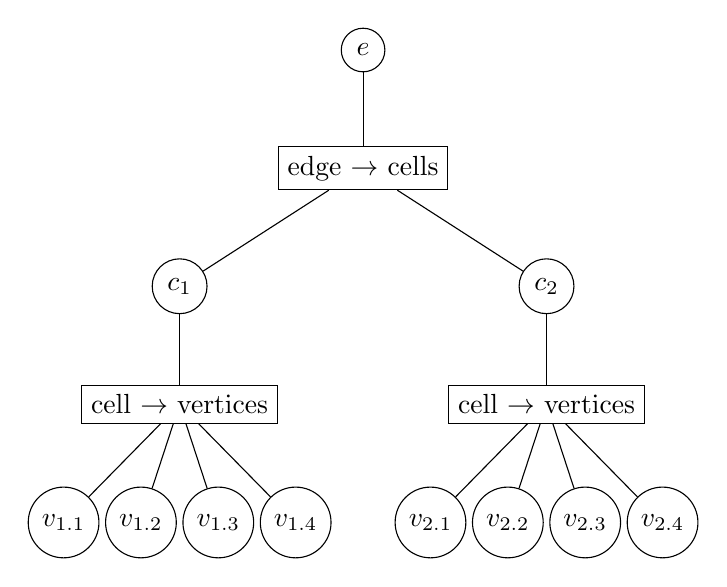
\begin{tikzpicture}[every tree node/.style={draw,circle},
        level distance=1.5cm,
        edge from parent path={(\tikzparentnode) -- (\tikzchildnode)}]

    \tikzset{level 2/.style={sibling distance=0.8cm}}

    \Tree
    [.{$e$}
        \edge node[auto=right] {\keyicon};
        [.\node[rectangle] {edge $\rightarrow$ cells};
            [.{$c_1$}
                \edge node[auto=right] {\keyicon};
                [.\node[rectangle] {cell $\rightarrow$ vertices};
                    [.$v_{1.1}$ ]
                    [.$v_{1.2}$ ]
                    [.$v_{1.3}$ ]
                    [.$v_{1.4}$ ]
                ]
            ]
            [.{$c_2$}
                \edge node[auto=right] {\keyicon};
                [.\node[rectangle] {cell $\rightarrow$ vertices};
                    [.$v_{2.1}$ ]
                    [.$v_{2.2}$ ]
                    [.$v_{2.3}$ ]
                    [.$v_{2.4}$ ]
                ]
            ]
        ]
    ]
    \end{tikzpicture}
    \caption{
    In this example, we consider a core-computation operating over the edge set, with $e$ being the indexing variable into the edge set.
    The edge $\rightarrow$ cells map is indexed by $e$ to obtain the the two cells $c_1$ and $c_2$ incident on the edge $e$. The cell $\rightarrow$ vertices map is then indexed by both $c_1$ and $c_2$ to obtain their respective vertices. The key symbol denotes indexing into the map below, using the indexing variable above.
    }
    \label{fig:relation-tree}
\end{figure}


\subsection{Given: kernel function}
\label{subsec:given-kernel-function}
We are given a kernel function specifying the computation logic, which is applied to each element in the operating set. It takes as arguments all gathered indexing variables, including that of the current element, and it has read and write access to the mesh's associated data. The access pattern of a kernel function is similar to that of a stencil computation, as defined by~\cite{tang2011pochoir}:
\begin{quote}
A stencil computation repeatedly updates each point of a d-dimensional grid as a function of itself and its near neighbours.
\end{quote}
As we define it, however, kernel functions are in fact more general than a stencil computation, as they access neighbouring elements across different operating sets.


The kernel function is applied to the operating set elements in no particular order; the indexing variables, however, are passed to the kernel in some known order, typically in the order stored in the relation-map.


\subsection{Expected operation}
Given all the above, a core-computation is then performed as follows:
\begin{enumerate}
\item Iterate over the elements of the operating set, in no particular order.
\item For each element iterated over:
    \begin{enumerate}
    \item Gather any indexing variables as defined by the relation-map tree. This may involve indexing variables obtained through a chain of relation-maps.
    \item Call the kernel function, passing the gathered indexing variables in some known order. The kernel function may access any associative data using these indexing variables.
    \end{enumerate}
\end{enumerate}



\section{Background on airfoils}
%% TODO CROSS REFERNCE to benchmarks
While not strictly needed for understanding our work, we nonetheless describe briefly airfoils and their function to offer a broader context. Much of this section was adapted from~\cite{abbott2012theory}, \cite{kuethe1986foundations} and~\cite{boeing2014airfoil}. Our description is nonetheless undoubtedly an overly simplistic one, and we would recommend that the aforementioned literature be sought for a fuller picture.

An airplane achieves flight by creating a lower air pressure over the wing (\emph{the upper surface}) whilst maintaining a higher air pressure below the wing (\emph{the lower surface}). The exact way in which this is achieved is characteristic of the wing shape as well as other factors. The pressure differential causes air in the lower surface to push towards the upper surface, creating a lift force. If the lift force is sufficient to counteract the gravitational force, the airplane flies.

An airfoil is the two-dimensional cross-section \emph{shape} of a wing. They are used to model the hydrodynamics (fluid motion) surrounding a particular wing shape in different contexts, including the velocity and angle of motion (known as the \emph{angle of attack}). Figure~\ref{fig:airfoil-crosscut} shows how the cross-section is taken, as well as the modelled air flow.

\begin{figure}
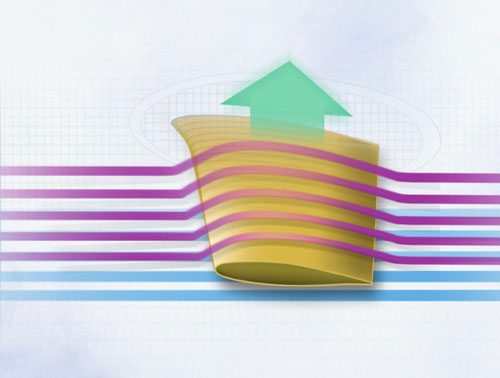
\includegraphics[width=\imagewidth]{images/background/airfoil_crosscut.jpg}
    \caption{The cross-section used to obtain the airfoil shape. Incoming air flow is split between the upper surface (purple) and the lower surface (blue). The image was obtained from~\cite{boeing2014airfoil}.}
    \label{fig:airfoil-crosscut}
\end{figure}


In 1929, the National Advisory Committee for Aeronautics (NACA) began to study various airfoils. They developed families of airfoil constructions parametrized by various geometric variables, depicted in figure~\ref{fig:airfoil-geometry}. We use specific instantiations of these airfoil families as benchmarks for Crystal.

\begin{figure}
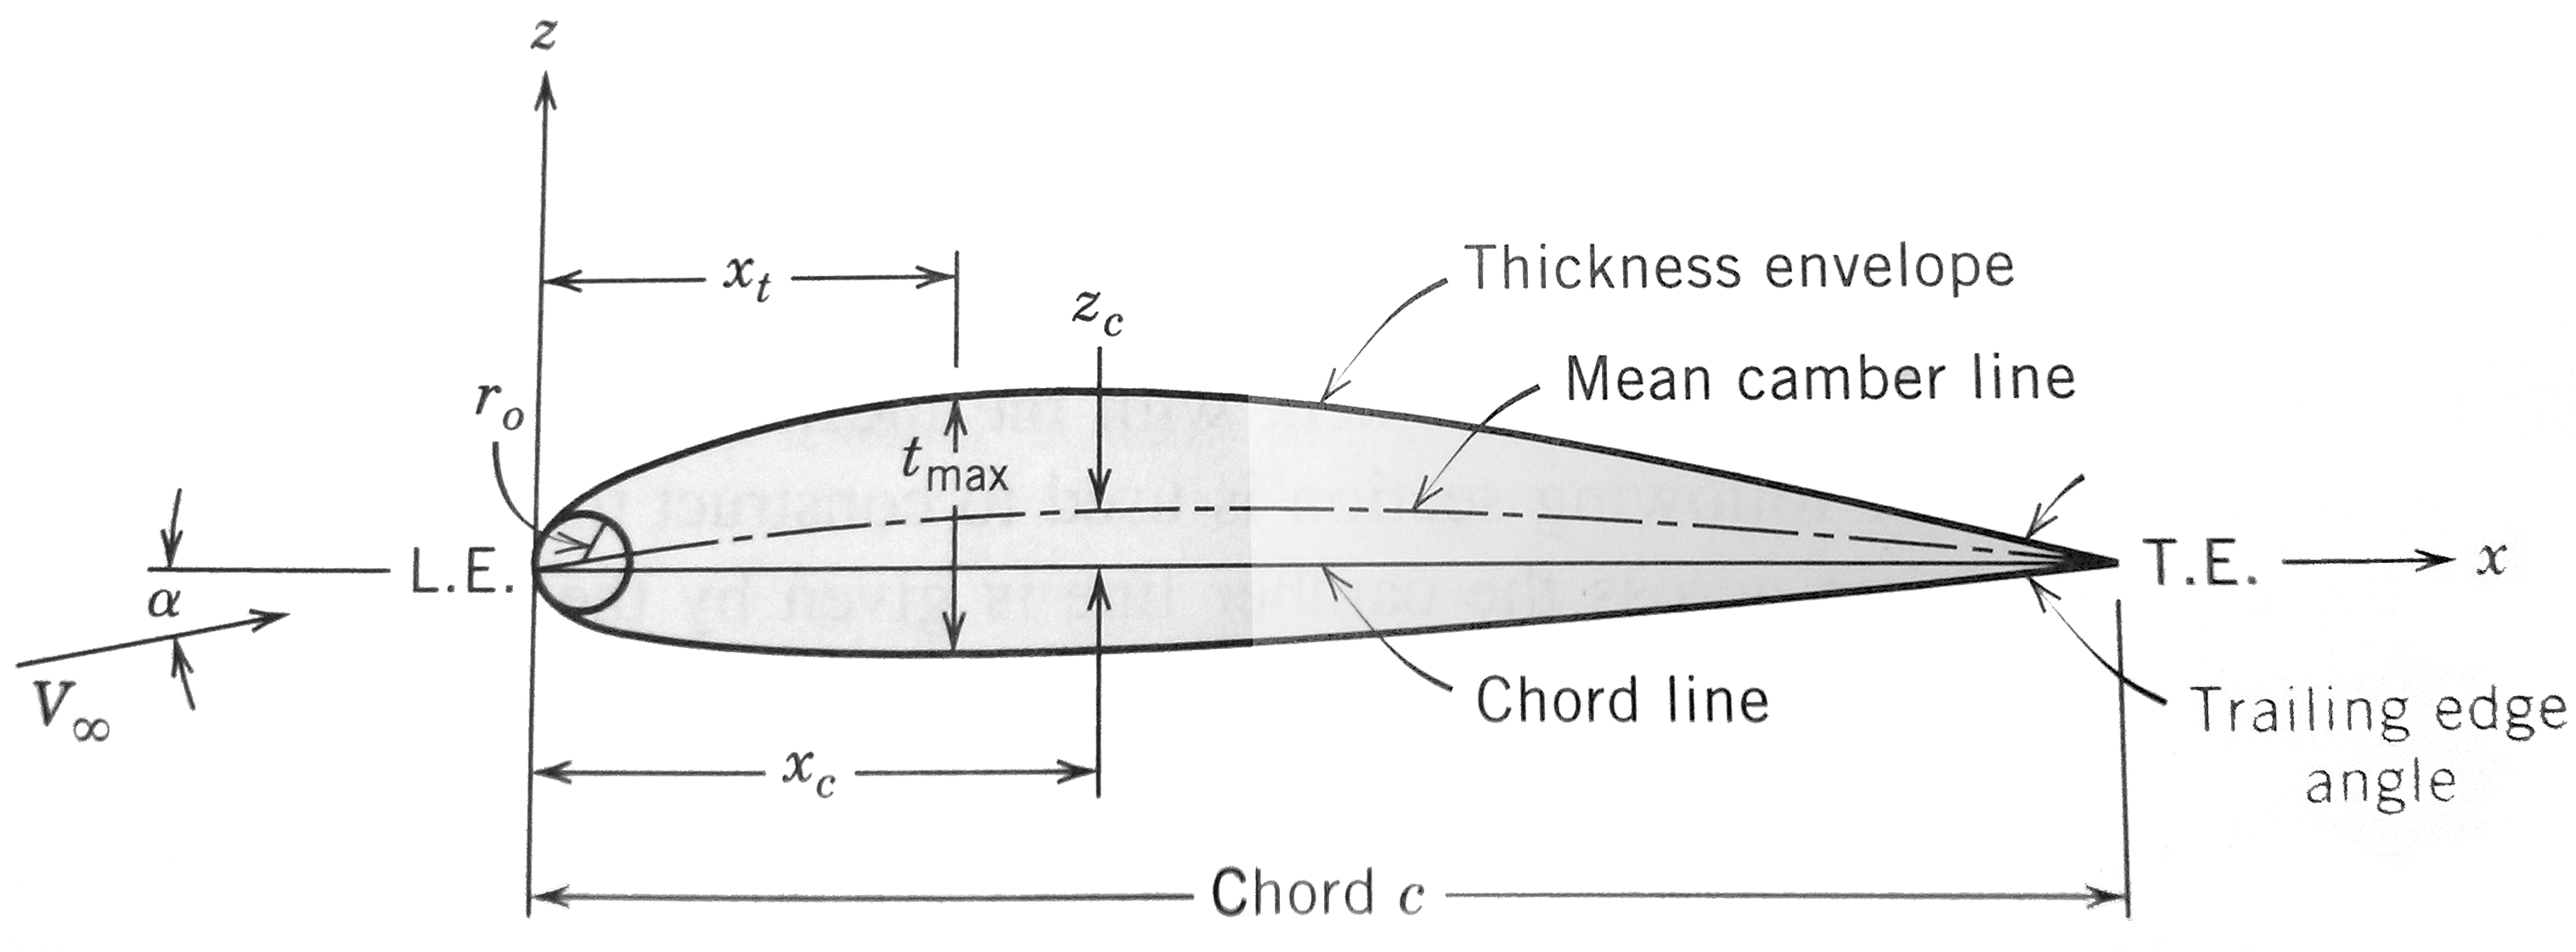
\includegraphics[width=\imagewidth]{images/background/airfoil.png}
    \caption{A depiction of the geometric properties of airfoil. The image was obtained from~\cite{kuethe1986foundations}.}
    \label{fig:airfoil-geometry}
\end{figure}

\section{Chapter summary}
In this chapter we gave a basic description of a mesh as a mathematical model. In addition we defined the concept of the mesh a data structure and how it is used in computation. Finally, we explained the significance of the airfoil in order to have a framing context for our running example.

\chapter{Diving into the problem}
\label{chap:diving-into-problem}
We begin by walking through an example mesh and examining the properties of the structure found within.

\section{A basic definition of structure}
What we would like is a form of structure which is
\begin{enumerate*}[label=\alph*)]
\item representable as a data structure, and \item efficient in terms of performance.
\end{enumerate*}

Given our semantic knowledge about the mesh model we can ascertain some facts about relation-maps:
\begin{itemize}
\item They are sparse: element arity is very small compared to the number of elements, and is in fact unrelated to it.
\item They have a high clustering coefficient: Relationships tend to be localized, forming tightly connected clusters.
% TODO REFERENCE TO CLUSTERING COEFFICIENTS
\end{itemize}

These properties arise as a consequence of meshes modelling real-world phenomena that exist in a Cartesian space.
On this basis, we consider a spatial embodiment of element relationships, organising the elements in a discrete space such that the uniform relationship is apparent.

Bear in mind that this approach carries no relation to any geometric data associated with elements, such as the coordinates of vertices. To make this distinction clear, as well as to emphasize its discrete nature, we address this Cartesian-like space by rows and columns rather than x and y coordinates.

\subsection{Example: Naca0012 mesh}
Figure~\ref{fig:naca12-plain} shows a small extract from the NACA0012 mesh\footnote{Thanks to Dr. Peter Vincent, George Ntemos and Harry Davis}, showing the cross section of an airfoil mesh and its interaction with surrounding fluid. The mesh is discretization into quadrilateral cells over which computations are performed.

\newcommand{\drawnaca}[4]{
	\begin{figure}
	\includesvg[svgpath=#1]{#2}
	\caption{#3}
	\label{#4}
	\end{figure}
}
\drawnaca{images/defining-structure/}{naca0012-plain}{Extract of the NACA0012 mesh.}{fig:naca12-plain}

The vertices in the highlighted region of figure~\ref{fig:naca12-vertices} seem like good candidates for a \emph{``structured region''}, forming a two-dimensional lattice in a discrete Cartesian space. This \emph{``structured region''} has the properties outlined below.

\drawnaca{images/defining-structure/}{naca0012-node-structure}{Highlighted vertices which exhibit a form of \emph{``structured region''}.}{fig:naca12-vertices}

\subsection{Desired properties of a structured region}
\label{sec:structured-region-properties}
\begin{enumerate}
\item All vertices have a uniform arity of four.
\item Every vertex has a consistent discrete direction (for example the cardinal directions: north east, south, west) with respect to the other vertices. In other words, the direction is transitive: if vertex $a$ is above vertex $b$, and vertex $b$ is above vertex $c$, then vertex $a$ is above vertex $c$. For a non-example see figure~\ref{fig:non-consistent-direction}.
\end{enumerate}

\begin{figure}
\includesvg[width=\imagewidth, svgpath=images/defining-structure/]{non-consistent-direction}
\caption{An example of inconsistent direction. We can traverse cells in \emph{``one direction''} by following the edge parallel to the one we entered from. If we start from $A$ and traverse the cells in one direction (the blue path) we reach $Z$. If we start from $A$ and traverse the cells in an orthogonal direction (the red path) to the first path, we also reach $Z$! Is $Z$ then \emph{``above''} $A$ or \emph{``to the side of it''}?}
\label{fig:non-consistent-direction}
\end{figure}


%% TODO Maybe not introduce data structure yet????
We can propagate this inherent structure from the mesh model to the underlying data structure, representing this two-dimensional lattice using a two-dimensional array. Vertices may be assigned Cartesian coordinates, but in spirit of the space's discreteness we shall use rows and columns instead. See figure~\ref{fig:naca12-structure-grid}.\label{sentence:2d-array}

\drawnaca{images/defining-structure/}{naca0012-node-grid}{The overlaid grid shows the lattice structure more clearly.}{fig:naca12-structure-grid}


\newcommand{\strV}{V_{str}}
\newcommand{\adjstrV}{V_{adjstr}}
\newcommand{\AdjVVstr}{Adj_{\adjstrV\strV}}

Let us call $\VertexSet$ the set of all vertices, and $\strV \subseteq \VertexSet$ the set of vertices in the \emph{``structured region''}.

\subsection{Representing the vertex-vertex adjacency}

Now consider the vertex-vertex adjacency relation $\AdjVV: \VertexSet \mapsto \VertexSet$ in context of the \emph{``structured region''} $\strV$. We can directly locate a particular neighbour of any vertex, for example its north neighbour, so long as that neighbour is also within the structured region. This restricts the set of vertices with fully-accessible neighbours to those which are not on the borders or the fringe of the \emph{``structured region''}. This is the subset of vertices $\adjstrV \subseteq \strV$ which are structured \emph{with respect to} $\AdjVV$. This induces a new relation which operates purely within the structured region:
$$\AdjVVstr: \adjstrV \mapsto \strV$$

Figures~\ref{fig:naca12-structured-highlighted} and~\ref{fig:structure-as-graph} illustrate these two sets.
\drawnaca{images/defining-structure/}{naca0012-node-neighbours}{The interior structured vertices (those not on the fringe) are highlighted in dark blue.}{fig:naca12-structured-highlighted}


\begin{figure}
% Draw structured node region
\begin{tikzpicture}[scale=0.7]
	\newcommand{\stylewithfill}[1]{\tikzstyle{every node}=[draw, shape=circle, minimum size=0.8cm, fill=#1];}
	\stylewithfill{none}

	% ROW 0
	\drawgrid{rows=1, cols=3, rowoffset=0, coloffset=4, labeler=\plainlabelnode, labelerA=0, labelerB=2,
		southborder=structured}

	% ROW 1
	\drawgrid{rows=1, cols=2, rowoffset=-2, coloffset=0, labeler=\plainlabelnode, labelerA=1, labelerB=0,
		eastborder=structured}

	{
	\stylewithfill{neighbourstructurecolor}
	\drawgrid{rows=1, cols=2, rowoffset=-2, coloffset=4, labeler=\plainlabelnode, labelerA=1, labelerB=2,
		northborder=structured, southborder=structured, westborder=structured, eastborder=structured}
	}

	\drawgrid{rows=1, cols=1, rowoffset=-2, coloffset=8, labeler=\plainlabelnode, labelerA=1, labelerB=4,
		northborder=structured, southborder=structured, westborder=structured}


	\drawgrid{rows=1, cols=1, rowoffset=-2, coloffset=12, labeler=\plainlabelnode, labelerA=1, labelerB=6,
		southborder=structured, eastborder=structured}

	\drawgrid{rows=1, cols=1, rowoffset=-2, coloffset=14, labeler=\plainlabelnode, labelerA=1, labelerB=7,
		westborder=structured}

	% ROW 2
	\drawgrid{rows=1, cols=1, rowoffset=-4, coloffset=4, labeler=\plainlabelnode, labelerA=2, labelerB=2,
		northborder=structured, southborder=structured, eastborder=structured}

	{
	\stylewithfill{neighbourstructurecolor}
	\drawgrid{rows=1, cols=2, rowoffset=-4, coloffset=6, labeler=\plainlabelnode, labelerA=2, labelerB=3,
		northborder=structured, southborder=structured, eastborder=structured, westborder=structured}
	}

	\drawgrid{rows=1, cols=1, rowoffset=-4, coloffset=10, labeler=\plainlabelnode, labelerA=2, labelerB=5,
		southborder=structured, westborder=structured, eastborder=structured}

	\drawgrid{rows=1, cols=1, rowoffset=-4, coloffset=12, labeler=\plainlabelnode, labelerA=2, labelerB=6,
		northborder=structured, westborder=structured}

	% ROW 3
	\drawgrid{rows=1, cols=1, rowoffset=-6, coloffset=4, labeler=\plainlabelnode, labelerA=3, labelerB=2,
		northborder=structured, southborder=structured, eastborder=structured}

	{
	\stylewithfill{neighbourstructurecolor}
	\drawgrid{rows=1, cols=2, rowoffset=-6, coloffset=6, labeler=\plainlabelnode, labelerA=3, labelerB=3,
		northborder=structured, southborder=structured, eastborder=structured, westborder=structured}
	}

	\drawgrid{rows=1, cols=1, rowoffset=-6, coloffset=10, labeler=\plainlabelnode, labelerA=3, labelerB=5,
		northborder=structured, westborder=structured}

	% ROW 4
	\drawgrid{rows=1, cols=1, rowoffset=-8, coloffset=2, labeler=\plainlabelnode, labelerA=4, labelerB=1, eastborder=structured}

	{
	\stylewithfill{neighbourstructurecolor}
	\drawgrid{rows=1, cols=2, rowoffset=-8, coloffset=4, labeler=\plainlabelnode, labelerA=4, labelerB=2,
		northborder=structured, southborder=structured, eastborder=structured, westborder=structured}
	}

	\drawgrid{rows=1, cols=1, rowoffset=-8, coloffset=8, labeler=\plainlabelnode, labelerA=4, labelerB=4,
		northborder=structured, westborder=structured}

	% ROW 5
	\drawgrid{rows=1, cols=2, rowoffset=-10, coloffset=4, labeler=\plainlabelnode, labelerA=5, labelerB=2,
		northborder=structured}
\end{tikzpicture}
\caption{The vertices in figure~\ref{fig:naca12-structured-highlighted} represented as a graph.}
\label{fig:structure-as-graph}
\end{figure}

The key insight we make is that for structured regions in a mesh we need not represent set relationship maps explicitly; the uniformity of set relations allows us to deduce the relationships. We can encode the relation $\AdjVVstr$ very simply. Given a vertex $n_{r,c} \in \adjstrV$, located at row $r$ and column $c$, its four vertex neighbours are $n_{r,c-1}$, $n_{r,c+1}$, $n_{r-1,c}$, and $n_{r+1,c}$. This is illustrated in figure~\ref{fig:single-vertex-neighbours}.



\begin{figure}
% Draw structured node region
\begin{tikzpicture}[scale=1]
	\newcommand{\stylewithfill}[1]{\tikzstyle{every node}=[draw, shape=circle, minimum size=1.3cm, fill=#1];}
	\stylewithfill{none}

	% ROW 0
	\drawgrid{rows=1, cols=1, rowoffset=0, coloffset=2,
		labeler=\varlabelnode, labelerA=-1, labelerB=0, labelerC=r, labelerD=c,
		southborder=structured}

	% ROW 1
	\drawgrid{rows=1, cols=1, rowoffset=-2, coloffset=0,
		labeler=\varlabelnode, labelerA=0, labelerB=-1, labelerC=r, labelerD=c,
		eastborder=structured}

	{
		\stylewithfill{neighbourstructurecolor}
		\drawgrid{rows=1, cols=1, rowoffset=-2, coloffset=2,
			labeler=\varlabelnode, labelerA=0, labelerB=0, labelerC=r, labelerD=c,
			eastborder=structured, westborder=structured, northborder=structured, southborder=structured}
	}

	\drawgrid{rows=1, cols=1, rowoffset=-2, coloffset=4,
		labeler=\varlabelnode, labelerA=0, labelerB=1, labelerC=r, labelerD=c,
		westborder=structured}

	% ROW 2
	\drawgrid{rows=1, cols=1, rowoffset=-4, coloffset=2,
		labeler=\varlabelnode, labelerA=1, labelerB=0, labelerC=r, labelerD=c,
		northborder=structured}

\end{tikzpicture}
\caption{The neighbours of a structured vertex.}
\label{fig:single-vertex-neighbours}
\end{figure}


\section{Mesh structure as a data structure}
The choice of data structure to represent the structured region is a key one, touching on various aspects:
\begin{itemize}
\item Scope of structure representation: what level of structure can be represented.
\item Implementation complexity of structure detection: how complex a detection algorithm is required.
\item Runtime performance of structure detection: the time and space complexity of the detection algorithm.
\item Storage requirements for detected structure: the storage requirements for the detected structure.
\item Runtime performance of computation over the structured region.
\end{itemize}

We analyse several possible data structure representations.

\subsection{Structure bit-mask}
\label{subsec:structure-bitmap}

\newcommand{\drawbitmap}[2]{
	% trim left bottom right top
	\includesvg[svgpath=#1]{#2}
}

Represent the bounding box around the structured region as a two-dimensional bit-mask, with each bit representing a vertex position in the superimposed grid. An \emph{on} bit indicates that the corresponding vertex is part of the structured region, an \emph{off} bit otherwise.

A bit-mask can represent \emph{any} structured region which adheres to the properties listed in section~\ref{sec:structured-region-properties}. They are very flexible, capable of representing complex formations as well as handling small anomalies in structure.

Let us define the \emph{efficiency} $\epsilon$ of a bit-mask as the percentage of its bits which are \emph{on}, as the \emph{off} bits represent wasted vertices. Bit-masks with high $\epsilon$ are favourable for several reasons:
\begin{itemize}
\item \emph{Off} bits increase the storage space of the structured region, up to $O(\card{\VertexSet})$ in the worst case, as opposed to $O(\card{\Structured})$.
\item \emph{Off} bits similarly worsen the runtime performance, again up to $O(\card{\VertexSet})$ due to wasted execution.
\end{itemize}

Figure~\ref{fig:example-bitmask} shows an example of a good bit-mask candidate.

\begin{figure}
\pgfplotstableread{
	1 1 1 1 1 1
	1 2 2 1 1 1
	1 1 2 1 1 2
	1 1 1 1 1 1
	1 1 1 1 1 2
	2 1 1 1 1 1
}{\bitmapmatrix}
\drawmatrix[cell wd=0.8, cell ht=0.8]{\bitmapmatrix}
\caption{An example of a structured region which can be bit-mask defined. The dotted regions indicate unstructured cells. The blue cells are structured cells. Its efficiency $\epsilon$ is $\frac{30}{36} \approx 83\%$.}
\label{fig:example-bitmask}
\end{figure}

A detection algorithm would likely be implemented using a variant of a general graph search algorithm such as breadth-first search or depth-first search. Further consolidation work may be needed to compact disconnected structured components in order to maximize $\epsilon$. The potential benefits of compaction are illustrated in figure~\ref{fig:disjoint-matrix}.

\begin{figure}
\pgfplotstableread{
	2 2 2 2 2 1
	1 2 2 2 2 1
	1 1 2 2 2 2
	2 1 2 2 2 2
	2 1 2 1 2 2
	2 1 1 1 2 2
}{\disjointAmatrix}
\pgfplotstableread{
	1 2 2 1
	1 1 2 1
	2 1 2 2
	2 1 2 1
	2 1 1 1
}{\disjointBmatrix}

\sidebyside
{
\drawmatrix[cell wd=0.8, cell ht=0.8]{\disjointAmatrix}
\caption{Originally detected structured components.}
\label{subfig:original-components}
}
{
\drawmatrix[cell wd=0.8, cell ht=0.8]{\disjointBmatrix}
\caption{Compacted structured components.}
\label{subfig:compacted-components}
}
\caption{A demonstration of the benefits of disconnect structured components compaction. The detected structured cell components in~\ref{subfig:original-components} are unnecessarily sparse and occupy more space than necessary. After compaction in~\ref{subfig:compacted-components} the space is used is reduced by over 40\%.}
\label{fig:disjoint-matrix}
\end{figure}


\subsection{Row-specific boundaries}

Represent the structured region as a sequence of consecutive fixed-length rows, permitting vertices outside the structured region to cluster at the beginning and ends of each row. A structured region is then represented by the row-length, as well as individual begin and end offsets for each row. This is exemplified in figure~\ref{fig:row-specific}.

\begin{figure}
\pgfplotstableread{
	0 2 1 1 1 1
	2 2 1 1 1 2
	1 1 1 1 2 0
	2 1 1 1 1 1
	1 1 1 1 1 1
	2 2 1 1 2 2
}{\bitmapmatrix}
\drawmatrix[cell wd=0.8, cell ht=0.8]{\bitmapmatrix}
\caption{An example of a structured region which can be represented using row-specific boundaries. Note the white cells, which represent unused structured regions near the boundaries.}
\label{fig:row-specific}
\end{figure}

Storing row-specific boundaries reduces the storage requirement by the order of row-length times.
No executions are wasted as the loop iterations are constrained to vertices in the structured region.
A detection algorithm can be implemented as a simple row-by-row traversal in linear time and space.


On the downside, this scheme trades some of the flexibility offered by the bit-mask representation, in particularly anomalies in structure which do not occur at the boundaries.


\subsection{Full rectangle}

Represent the structured region as a rectangle of given length and width, with all elements corresponding strictly to vertices within the structured region. The structured region is thus simply represented by the length and the width: the number of rows and the number of columns. Figure~\ref{fig:rectangle} shows an example of a rectangle-representable structured region.

The storage requirement is now constant with respect to the size of the structured region.
Loop iterations are fixed for each region, enabling further optimisation opportunities.
A detection algorithm, as above, can be implemented as a simple row-by-row traversal.

On the downside, the scope of structure representable is limited, being only capable of representing rectangles proper. Nonetheless, we stick with detecting rectangular structured regions for the remainder of this work as it seems to be the most promising choice.

\begin{figure}
\pgfplotstableread{
	0 2 2 0 2 0
	2 2 1 1 2 2
	2 0 1 1 2 2
	2 2 1 1 0 0
	0 2 1 1 2 2
	2 2 1 1 2 2
}{\bitmapmatrix}
\drawmatrix[cell wd=0.8, cell ht=0.8]{\bitmapmatrix}
\caption{An example of a rectangular structured region. Note the abundance of unused structured cells.}
\label{fig:rectangle}
\end{figure}

\section{Chapter summary}
In this chapter we derived intuitive definitions structure in a mesh in light of an excerpt from an airfoil mesh. We also discussed different representations in which they can be manifested, and the advantages and disadvantages of each.

\chapter{Structure Extraction}
\label{chap:detect-quad-grid}
Taking forth our length-first search algorithm, we expand fill in the details glossed over by our earlier discussion, delineating it into a formal algorithmic specification.

% Initial vertex
\newcommand{\vinit}{v_{init}}

\newcommand{\Quad}[4]{\begin{bmatrix} #1 & #2 \\ #3 & #4 \end{bmatrix}}

% Initial quad
\newcommand{\Qinit}{\Quad{n_{1,1}} {n_{1,2}} {n_{2,1}} {n_{2,2}} }

% Initial quad mirrored about y-axis
\newcommand{\Qinitmirror}{\Quad {n_{1,2}} {n_{1,1}} {n_{2,2}} {n_{2,1}}}



\section{Inputs}
\begin{enumerate}
\item A non-reflexive and symmetric vertex-vertex adjacency relation:
$$ \AdjVV: \VertexSet \mapsto \powerset{\VertexSet} $$

\item A set of visited vertices
$$ \Visited \subseteq \VertexSet $$

\item An unvisited start vertex
$$ \vinit \in \VertexSet \setminus \Visited $$
\end{enumerate}


\section{Outputs}
\begin{enumerate}
\item A structured set of vertices $\Structured \subseteq \VertexSet \setminus \Visited $ forming the extracted structured region.
The vertices $\Structured$ are structured on a 2-dimensional Cartesian lattice with $m$ rows and $n$ columns.
\end{enumerate}


%%%% PHASE 1

%% Phase 1 summary
\section{Phase 1: Grow a quad}
\label{sec:grow_a_quad}
Starting from the initial vertex $\vinit$, call it $n_{1,1}$, we would like to discover three other vertices $n_{1,2}$, $n_{2,1}$, and $n_{2,2}$ such that $\Qinit$ forms a valid quad in a structured quad region. They must satisfy the following constraints:

\begin{itemize}
\item Each of the four vertices must have exactly 4 neighbours.
\item Each of the following pairs of vertices are neighbours: $n_{1,1}$~and~$n_{1,2}$ ; $n_{1,2}$~and~$n_{2,2}$ ; $n_{2,2}$~and~$n_{2,1}$ ; $n_{2,1}$~and~$n_{1,1}$.
\item Each of the vertices must \emph{not} neighbour any vertex that has been visited thus far, apart from those vertices explicitly mentioned.
\end{itemize}

%% Phase 1 diagram

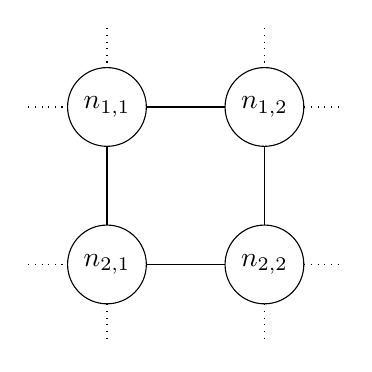
\begin{tikzpicture}[scale=1]
	% Default action for each node
	\tikzstyle{every node}=[draw, shape=circle, minimum size=1cm];

										\coordinate (northleft) at (0, 2);	\coordinate (northright) at (2, 2);
	\coordinate (westup) at (-1,1);		\node (r1c1) at (0,1) {$n_{1,1}$};	\node (r1c2) at (2,1) {$n_{1,2}$};	\coordinate (eastup) at (3,1);
	\coordinate (westdown) at (-1,-1);	\node (r2c1) at (0,-1) {$n_{2,1}$};	\node (r2c2) at (2,-1) {$n_{2,2}$};	\coordinate (eastdown) at (3,-1);
										\coordinate (southleft) at (0, -2);	\coordinate (southright) at (2, -2);

	% Horizontals
	\draw[outside] (westup) -- (r1c1);
	\draw (r1c1) -- (r1c2);
	\draw[outside] (r1c2) -- (eastup);

	\draw[outside] (westdown) -- (r2c1);
	\draw (r2c1) -- (r2c2);
	\draw[outside] (r2c2) -- (eastdown);

	% Verticals
	\draw[outside] (northleft) -- (r1c1);
	\draw (r1c1) -- (r2c1);
	\draw[outside] (r2c1) -- (southleft);

	\draw[outside] (northright) -- (r1c2);
	\draw (r1c2) -- (r2c2);
	\draw[outside] (r2c2) -- (southright);
\end{tikzpicture}

%% Phase 1 algorithm

\subsection{Algorithm}

\begin{enumerate}
\item If $\vinit$ does not have exactly 4 neighbours, that is $ \card{\AdjVV(\vinit)} \neq 4 $, return immediately with $\Structured = \varnothing$.
\item Let $ n_{1,1} = \vinit $, and let $ a, b, c \in \AdjVV(\vinit) $ be distinct vertex neighbours of $\vinit$. Consider vertices $a$ and $b$. If they do not both have exactly 4 neighbours, then they cannot form a part of a structured quad region. Return immediately with $\Structured = \varnothing$.

\item Otherwise, there are three cases:

	%%%% BEGIN THREE CASES
	\begin{enumerate}

	%% Straight line case
	\item $a$ and $b$ have exactly one neighbour in common, which must be $n_{1,1}$ by construction, expressed by:
	$$ \card{\AdjVV(a) \cap \AdjVV(b)} = 1$$
	$a, n_{1,1}, b $ are \emph{topologically} along a straight line of a structured grid, and hence cannot form a quad.
	We therefore consider $b$, $n_{1,1}$, and  $c$ instead as candidates, letting $n_{2,1} = b$ and $n_{1,2} = c$.
	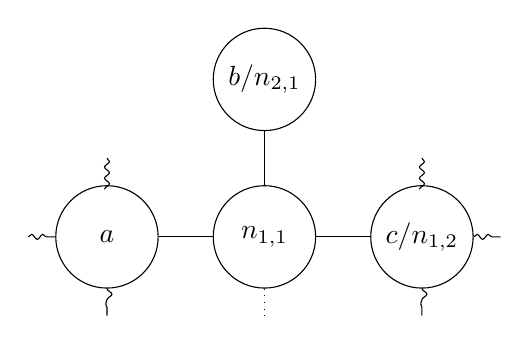
\begin{tikzpicture}
		% Default action for each node
		\tikzstyle{every node}=[draw, shape=circle, minimum size=1.3cm];

										\coordinate (northleft) at (-1,2);	\node (b) at (1,3) {$b / n_{2,1}$};	\coordinate (northright) at (3,2);
		\coordinate (west) at (-2,1);	\node (a) at (-1,1) {$a$};			\node (n11) at (1,1) {$n_{1,1}$};	\node (c) at (3,1) {$c / n_{1,2}$};	\coordinate (east) at (4,1);
										\coordinate (southleft) at (-1,0);	\coordinate (southmid) at (1,0);	\coordinate (southright) at (3,0);

		% Horizontals
		\draw[anywhere] (west) -- (a);
		\draw (a) -- (n11) -- (c);
		\draw[anywhere] (c) -- (east);

		% Verticals
		\draw[anywhere] (northleft) -- (a) -- (southleft);
		\draw (b) -- (n11);
		\draw[outside] (n11) -- (southmid);
		\draw[anywhere] (northright) -- (c) -- (southright);
	\end{tikzpicture}


	%% Angle case
	\item $a$ and $b$ have exactly two neighbours in common, one of which must be $n_{1,1}$ by construction, expressed by:
	$$ \card{\AdjVV(a) \cap \AdjVV(b)} = 2$$
	We continue with vertices $a$, $n_{1,1}$, and $b$ as candidates, letting $n_{2,1} = a$ and $n_{1,2} = b$.
	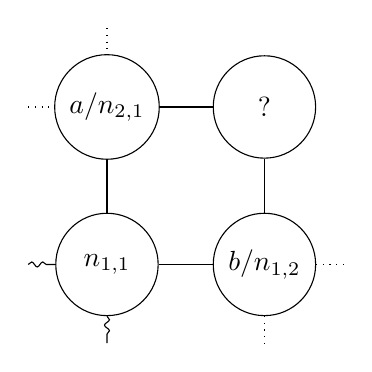
\begin{tikzpicture}
		% Default action for each node
		\tikzstyle{every node}=[draw, shape=circle, minimum size=1.3cm];

											\coordinate (northleft) at (-1,4);		\coordinate (northright) at (1,4);
		\coordinate (westup) at (-2,3);		\node (a) at (-1,3) {$a / n_{2,1}$};	\node (d) at (1,3) {$?$};			\coordinate (eastup) at (2,3);
		\coordinate (westdown) at (-2,1);	\node (n11) at (-1,1) {$n_{1,1}$};		\node (b) at (1,1) {$b / n_{1,2}$};	\coordinate (eastdown) at (2,1);
											\coordinate (southleft) at (-1,0);		\coordinate (southright) at (1,0);



		\draw[outside] (westup) -- (a);
		\draw (a) -- (d);
		% \draw (d) -- (eastup);

		\draw[anywhere] (westdown) -- (n11);
		\draw (n11) -- (b);
		\draw[outside] (b) -- (eastdown);

		\draw[outside] (northleft) -- (a);
		\draw (a) -- (n11);
		\draw[anywhere] (n11) -- (southleft);

		% \draw (northright) -- (d);
		\draw (d) -- (b);
		\draw[outside] (b) -- (southright);

	\end{tikzpicture}


	\item $a$ and $b$ have more than two neighbours in common\footnote{Note that the set is non-empty by construction}, expressed by:
	$$ \card{\AdjVV(a) \cap \AdjVV(b)} > 2$$
	We cannot form a quad, and hence return immediately with $\Structured = \varnothing$.

	\end{enumerate}
	%%%% END THREE CASES

\item Find the common neighbours of $n_{2,1}$ and $n_{1,2}$. If these are not exactly two neighbours, return immediately with $\Structured = \varnothing$.

\item One of the two neighbours must be $n_{1,1}$ by construction. Let the other neighbour be $n_{2,2}$.

\item Let $N = \{ n_{1,1}, n_{1,2}, n_{2,1}, n_{2,2} \}$. If any vertex $n \in N$ is in $\Visited$, that is $N \cap \Visited \neq \varnothing$, then return immediately with $\Structured = \varnothing$. Otherwise add the vertices in $N$ to $\Visited$.

\item Ensure for every vertex $n \in N$ that its visited neighbours, $\AdjVV(n) \cap \Visited$, are exactly those explicitly stated above. If this is not the case, remove $N$ from $\Visited$ and return immediately with $\Structured = \varnothing$.


\item Set $\Structured = \Qinit$, and continue to the next phase.

The structured region looks as follows thus far.
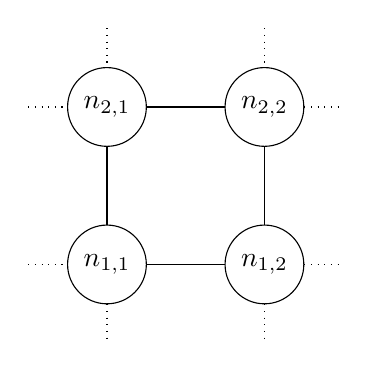
\begin{tikzpicture}
	% Default action for each node
	\tikzstyle{every node}=[draw, shape=circle, minimum size=1cm];

										\coordinate (northleft) at (-1,4);	\coordinate (northright) at (1,4);
	\coordinate (westup) at (-2,3);		\node (n21) at (-1,3) {$n_{2,1}$};	\node (n22) at (1,3) {$n_{2,2}$};	\coordinate (eastup) at (2,3);
	\coordinate (westdown) at (-2,1);	\node (n11) at (-1,1) {$n_{1,1}$};	\node (n12) at (1,1) {$n_{1,2}$};	\coordinate (eastdown) at (2,1);
										\coordinate (southleft) at (-1,0);	\coordinate (southright) at (1,0);

	\draw[outside] (westup) -- (n21);
	\draw (n21) -- (n22);
	\draw[outside] (n22) -- (eastup);

	\draw[outside] (westdown) -- (n11);
	\draw (n11) -- (n12);
	\draw[outside] (n12) -- (eastdown);

	\draw[outside] (northleft) -- (n21);
	\draw (n21) -- (n11);
	\draw[outside] (n11) -- (southleft);

	\draw[outside] (northright) -- (n22);
	\draw (n22) -- (n12);
	\draw[outside] (n12) -- (southright);

\end{tikzpicture}

\end{enumerate}








%%%% Definition A

%% Definition A summary
\section{Function definition: Extend a quad (used in phase 2)}
Starting from $Q_i = \Quad {n_{1,i}} {n_{1,i+1}} {n_{2,i}} {n_{2,i+1}}$, which must be a valid quad in a structured region, we would like to find two more vertices $n_{1, i+2}$ and $n_{2,i+2}$, such that $Q_{i+1} = \Quad {n_{1,i+1}} {n_{1,i+2}} {n_{2,i+1}} {n_{2,i+2}}$ forms a valid quad in a structured quad region. They must satisfy the following constraints:

\begin{itemize}
\item Each of the vertices $n_{1, i+2}$ and $n_{2,i+2}$ must have exactly 4 neighbours.
\item Each of the following pairs of vertices are neighbours: $n_{1,i+1}$~and~$n_{1,i+2}$ ; $n_{2,i+1}$~and~$n_{2,i+2}$ ; $n_{1,i+2}$~and~$n_{2,i+2}$.
\item Each of the vertices $n_{1, i+2}$ and $n_{2,i+2}$ must \emph{not} neighbour any vertex that has been visited thus far, apart from those vertices explicitly mentioned.
\end{itemize}

%% Definition A diagram

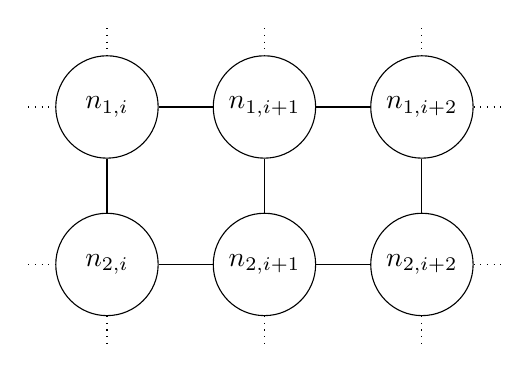
\begin{tikzpicture}[scale=1]
	% Default action for each node
	\tikzstyle{every node}=[draw, shape=circle, minimum size=1.3cm];

										\coordinate (northleft) at (0, 2);	\coordinate (northmid) at (2, 2);		\coordinate (northright) at (4, 2);
	\coordinate (westup) at (-1,1);		\node (r1c1) at (0,1) {$n_{1,i}$};	\node (r1c2) at (2,1) {$n_{1,i+1}$};	\node (r1c3) at (4,1) {$n_{1,i+2}$};	\coordinate (eastup) at (5,1);
	\coordinate (westdown) at (-1,-1);	\node (r2c1) at (0,-1) {$n_{2,i}$};	\node (r2c2) at (2,-1) {$n_{2,i+1}$};	\node (r2c3) at (4,-1) {$n_{2,i+2}$};	\coordinate (eastdown) at (5,-1);
										\coordinate (southleft) at (0, -2);	\coordinate (southmid) at (2, -2);		\coordinate (southright) at (4, -2);

	% Horizontals
	\draw[outside] (westup) -- (r1c1);
	\draw (r1c1) -- (r1c2);
	\draw (r1c2) -- (r1c3);
	\draw[outside] (r1c3) -- (eastup);

	\draw[outside] (westdown) -- (r2c1);
	\draw (r2c1) -- (r2c2);
	\draw (r2c2) -- (r2c3);
	\draw[outside] (r2c3) -- (eastdown);

	% Verticals
	\draw[outside] (northleft) -- (r1c1);
	\draw (r1c1) -- (r2c1);
	\draw[outside] (r2c1) -- (southleft);

	\draw[outside] (northmid) -- (r1c2);
	\draw (r1c2) -- (r2c2);
	\draw[outside] (r2c2) -- (southmid);

	\draw[outside] (northright) -- (r1c3);
	\draw (r1c3) -- (r2c3);
	\draw[outside] (r2c3) -- (southright);
\end{tikzpicture}


%% Definition A algorithm

\subsection{Algorithm}

\begin{enumerate}
\item $n_{1,i+1}$ has 4 neighbours, which include $n_{1,i}$ and $n_{2,i+1}$. Call the remaining 2 neighbours $a$ and $b$. This is expressed by:
$$ \AdjVV(n_{1,i+1}) \setminus \{ n_{1,i} , n_{2,i+1} \} = \{ a , b \} $$

\item $n_{2,i+1}$ has 4 neighbours, which include $n_{2,i}$ and $n_{1,i+1}$. Call the remaining 2 neighbours $c$ and $d$.
$$ \AdjVV(n_{2,i+1}) \setminus \{ n_{2,i} , n_{1,i+1} \} = \{ c , d \} $$

\item Choose two vertices $n_{1,i+2} \in \{ a , b \}$ and $n_{2,i+2} \in \{ c , d \}$ such that $n_{1,i+2}$ and $n_{2,i+2}$ are neighbours, which is expressible\footnote{Or equivalently (by symmetry of $\AdjVV$) $n_{2,i+2} \in \AdjVV(n_{1,i+2})$} as:
$$n_{1,i+2} \in \AdjVV(n_{2,i+2})$$
and such that they each have exactly 4 neighbours. If no such vertices $n_{1,i+2}$ and $n_{2,i+2}$ exist, fail the procedure.


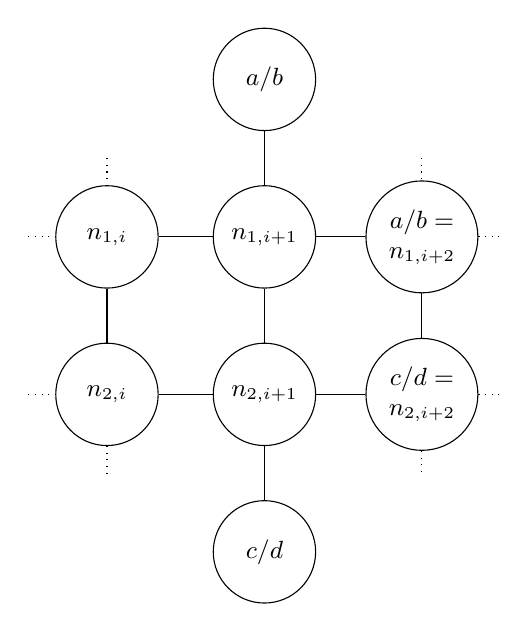
\begin{tikzpicture}[scale=1]
	% Default action for each node
	\tikzstyle{every node}=[draw, shape=circle, minimum size=1.3cm, align=center, font=\small];

										\coordinate (northleft) at (0, 2);	\coordinate (northmid) at (2, 2);		\coordinate (northright) at (4, 2);
	\coordinate (westup) at (-1,3);											\node (abup) at (2,3) {$a/b$};			\coordinate (eastup) at (5,1);
	\coordinate (westmid) at (-1,1);	\node (r1c1) at (0,1) {$n_{1,i}$};	\node (r1c2) at (2,1) {$n_{1,i+1}$};	\node (r1c3) at (4,1) {$a/b =$ \\ $n_{1,i+2}$};		\coordinate (eastmid) at (5,1);
	\coordinate (westdown) at (-1,-1);	\node (r2c1) at (0,-1) {$n_{2,i}$};	\node (r2c2) at (2,-1) {$n_{2,i+1}$};	\node (r2c3) at (4,-1) {$c/d =$ \\ $n_{2,i+2}$};	\coordinate (eastdown) at (5,-1);
	\coordinate (westlow) at (-1,-3);										\node (cdup) at (2,-3) {$c/d$};			\coordinate (eastlow) at (5,1);
										\coordinate (southleft) at (0, -2);	\coordinate (southmid) at (2, -2);		\coordinate (southright) at (4, -2);

	% Horizontals
	\draw[outside] (westmid) -- (r1c1);
	\draw (r1c1) -- (r1c2);
	\draw (r1c2) -- (r1c3);
	\draw[outside] (r1c3) -- (eastmid);

	\draw[outside] (westdown) -- (r2c1);
	\draw (r2c1) -- (r2c2);
	\draw (r2c2) -- (r2c3);
	\draw[outside] (r2c3) -- (eastdown);

	% Verticals
	\draw[outside] (northleft) -- (r1c1);
	\draw (r1c1) -- (r2c1);
	\draw[outside] (r2c1) -- (southleft);

	\draw (abup) -- (r1c2);
	\draw (r1c2) -- (r2c2);
	\draw (r2c2) -- (cdup);

	\draw[outside] (northright) -- (r1c3);
	\draw (r1c3) -- (r2c3);
	\draw[outside] (r2c3) -- (southright);
\end{tikzpicture}


\item If any of the two vertices $n_{1,i+2}$ and $n_{2,i+2}$ exists in $\Visited$, that is $\{ n_{1,i+2} , n_{2,i+2} \} \cap \Visited \neq \varnothing$, fail the procedure.
Otherwise add the two vertices to $\Visited$.

\item Ensure for every vertex $n \in \{ n_{1,i+2} , n_{2,i+2} \}$ that its visited neighbours, $\AdjVV(n) \cap \Visited$, are exactly those explicitly stated above. If this is not the case, remove $\{ n_{1,i+2} , n_{2,i+2} \}$ from $\Visited$ and fail the procedure.

\item Return the two vertices $n_{1,i+2}$ and $n_{2,i+2}$.
\end{enumerate}







%%%% PHASE 2

\section{Phase 2: Extend a row}
%% Phase 2.1 summary
``Extend a quad'' is iteratively applied, starting from $Q_1 = \Qinit$, to yield successive quads until it fails.
The resulting vertices are appended to the \emph{right} of $\Structured$ to form a single quad row in a structured quad region, or equivalently a successive pair of node rows.

%% Phase 2.1 diagram
\begin{tikzpicture}[scale=1]
	% Default action for each node
	\tikzstyle{every node}=[draw, shape=circle, minimum size=1.3cm];

	% MIDDLE

										\coordinate (northleft) at (0, 2);	\coordinate (northright) at (2, 2);
	\coordinate (westup) at (-1,1);		\node (r1c1) at (0,1) {$n_{1,1}$};	\node (r1c2) at (2,1) {$n_{1,2}$};		\coordinate (eastup) at (3,1);
	\coordinate (westdown) at (-1,-1);	\node (r2c1) at (0,-1) {$n_{2,1}$};	\node (r2c2) at (2,-1) {$n_{2,2}$};		\coordinate (eastdown) at (3,-1);
										\coordinate (southleft) at (0, -2);	\coordinate (southright) at (2, -2);

	% ellipses
	\coordinate (ellipsis westup) at (4,1);		\coordinate (ellipsis eastup) at (4.5,1);
	\coordinate (ellipsis westdown) at (4,-1);	\coordinate (ellipsis eastdown) at (4.5,-1);


	% RHS
											\coordinate (rhs north) at (6, 2);
	\coordinate (rhs westup) at (5,1);		\node (r1cn) at (6,1) {$n_{1,c_+}$};	\coordinate (rhs eastup) at (7,1);
	\coordinate (rhs westdown) at (5,-1);	\node (r2cn) at (6,-1) {$n_{2,c_+}$};	\coordinate (rhs eastdown) at (7,-1);
											\coordinate (rhs south) at (6, -2);



	% Horizontals
	\draw[outside] (westup) -- (r1c1);
	\draw (r1c1) -- (r1c2);
	\draw (r1c2) -- (r1c3);
	\draw (r1c3) -- (eastup);

	\draw[outside] (westdown) -- (r2c1);
	\draw (r2c1) -- (r2c2);
	\draw (r2c2) -- (r2c3);
	\draw (r2c3) -- (eastdown);

	\draw[ellipsis] (ellipsis westup) -- (ellipsis eastup);
	\draw[ellipsis] (ellipsis westdown) -- (ellipsis eastdown);


	\draw (rhs westup) -- (r1cn);
	\draw[outside] (r1cn) -- (rhs eastup);

	\draw (rhs westdown) -- (r2cn);
	\draw[outside] (r2cn) -- (rhs eastdown);

	% Verticals
	\draw[outside] (northleft) -- (r1c1);
	\draw (r1c1) -- (r2c1);
	\draw[outside] (r2c1) -- (southleft);

	\draw[outside] (northright) -- (r1c2);
	\draw (r1c2) -- (r2c2);
	\draw[outside] (r2c2) -- (southright);

	\draw[outside] (rhs north) -- (r1cn);
	\draw (r1cn) -- (r2cn);
	\draw[outside] (r2cn) -- (rhs south);
\end{tikzpicture}



%% Phase 2.2 summary
Next, ``Extend a quad'' is again iteratively applied, this time with $Q_1 = \Qinitmirror$, the mirror image of $Q_{init}$ about the y-axis.
The repeated application yields successive quads until the procedure fails.
The resulting vertices are appended to the \emph{left} of $\Structured$ to extend the existing quad row, or equivalently a successive pair of node rows.


%% Phase 2.2 diagram
\begin{tikzpicture}[scale=1]
	% Default action for each node
	\tikzstyle{every node}=[draw, shape=circle, minimum size=1.3cm];

	% LHS
												\coordinate (lhs north) at (-3.5, 2);
	\coordinate (lhs westup) at (-4.5,1);		\node (r1cm) at (-3.5,1) {$n_{1,c_{\!^{\_}}}$};		\coordinate (lhs eastup) at (-2.5,1);
	\coordinate (lhs westdown) at (-4.5,-1);	\node (r2cm) at (-3.5,-1) {$n_{2,c_{\!^{\_}}}$};	\coordinate (lhs eastdown) at (-2.5,-1);
												\coordinate (lhs south) at (-3.5, -2);

	% lhs ellipses
	\coordinate (lhs ellipsis westup) at (-2,1);	\coordinate (lhs ellipsis eastup) at (-1.5,1);
	\coordinate (lhs ellipsis westdown) at (-2,-1);	\coordinate (lhs ellipsis eastdown) at (-1.5,-1);


	% MIDDLE
										\coordinate (northleft) at (0, 2);	\coordinate (northright) at (2, 2);
	\coordinate (westup) at (-1,1);		\node (r1c1) at (0,1) {$n_{1,1}$};	\node (r1c2) at (2,1) {$n_{1,2}$};		\coordinate (eastup) at (3,1);
	\coordinate (westdown) at (-1,-1);	\node (r2c1) at (0,-1) {$n_{2,1}$};	\node (r2c2) at (2,-1) {$n_{2,2}$};		\coordinate (eastdown) at (3,-1);
										\coordinate (southleft) at (0, -2);	\coordinate (southright) at (2, -2);

	% rhs ellipses
	\coordinate (rhs ellipsis westup) at (4,1);		\coordinate (rhs ellipsis eastup) at (4.5,1);
	\coordinate (rhs ellipsis westdown) at (4,-1);	\coordinate (rhs ellipsis eastdown) at (4.5,-1);


	% RHS
											\coordinate (rhs north) at (6, 2);
	\coordinate (rhs westup) at (5,1);		\node (r1cn) at (6,1) {$n_{1,c_+}$};	\coordinate (rhs eastup) at (7,1);
	\coordinate (rhs westdown) at (5,-1);	\node (r2cn) at (6,-1) {$n_{2,c_+}$};	\coordinate (rhs eastdown) at (7,-1);
											\coordinate (rhs south) at (6, -2);



	% Horizontals
	\draw (westup) -- (r1c1);
	\draw (r1c1) -- (r1c2);
	\draw (r1c2) -- (r1c3);
	\draw (r1c3) -- (eastup);

	\draw(westdown) -- (r2c1);
	\draw (r2c1) -- (r2c2);
	\draw (r2c2) -- (r2c3);
	\draw (r2c3) -- (eastdown);


	\draw[ellipsis] (rhs ellipsis westup) -- (rhs ellipsis eastup);
	\draw[ellipsis] (rhs ellipsis westdown) -- (rhs ellipsis eastdown);

	\draw (rhs westup) -- (r1cn);
	\draw[outside] (r1cn) -- (rhs eastup);

	\draw (rhs westdown) -- (r2cn);
	\draw[outside] (r2cn) -- (rhs eastdown);


	\draw[ellipsis] (lhs ellipsis westup) -- (lhs ellipsis eastup);
	\draw[ellipsis] (lhs ellipsis westdown) -- (lhs ellipsis eastdown);

	\draw (r1cm) -- (lhs eastup);
	\draw[outside] (lhs westup) -- (r1cm);

	\draw[outside] (lhs westdown) -- (r2cm);
	\draw (r2cm) -- (lhs eastdown);


	% Verticals
	\draw[outside] (northleft) -- (r1c1);
	\draw (r1c1) -- (r2c1);
	\draw[outside] (r2c1) -- (southleft);

	\draw[outside] (northright) -- (r1c2);
	\draw (r1c2) -- (r2c2);
	\draw[outside] (r2c2) -- (southright);


	\draw[outside] (rhs north) -- (r1cn);
	\draw (r1cn) -- (r2cn);
	\draw[outside] (r2cn) -- (rhs south);


	\draw[outside] (lhs north) -- (r1cm);
	\draw (r1cm) -- (r2cm);
	\draw[outside] (r2cm) -- (lhs south);
\end{tikzpicture}












%% Phase 2 algorithm

\subsection{Algorithm}

\paragraph{Extend to the right}
\begin{enumerate}
\item Let $Q_{in} = Q_{init} = \Qinit$, as produced by ``Grow a quad''.
\item \label{step:extend_quad} Let $\Quad {n_{1,i}} {n_{1,i+1}} {n_{2,i}} {n_{2,i+1}}$ represent the elements of $Q_{in}$.
\item Call the procedure ``Extend a quad'' with $Q_{in}$ as input.
\item If the procedure fails, go to step~\ref{step:init_reverse}.
\item Otherwise, append the two new vertices obtained, $n_{1,i+2}$ and $n_{2,i+2}$ to the \emph{right} of $\Structured$. \\
Thus $\Structured$ will become:
	$\begin{bmatrix}
	n_{1,1} & n_{1,2} & \cdots  & n_{1,i} & n_{1,i+1} & n_{1,i+2} \\
	n_{2,1} & n_{2,2} & \cdots  & n_{2,i} & n_{2,i+1} & n_{2,i+2}
	\end{bmatrix}$

\item Set $Q_{in} = \Quad {n_{1,i+1}} {n_{1,i+2}} {n_{2,i+1}} {n_{2,i+2}}$, and continue from step~\ref{step:extend_quad}.

\end{enumerate}
\paragraph{Extend to the left}
\begin{enumerate}[resume]

% Reverse
\item \label{step:init_reverse} Let $Q_{in} = \Qinitmirror$ be the mirror image of $Q_{init}$ about the y-axis.



\item \label{step:reverse_extend_quad} Let $\Quad {n_{1,i}} {n_{1,i+1}} {n_{2,i}} {n_{2,i+1}}$ represent the elements of $Q_{in}$.
\item Call the procedure ``Extend a quad'' with $Q_{in}$ as input.
\item If the procedure fails, return immediately.
\item Otherwise, append the two new vertices obtained, $n_{1,i+2}$ and $n_{2,i+2}$ to the \emph{left} of $\Structured$. \\
Thus $\Structured$ will become:
	$\begin{bmatrix}
	n_{1,i+2} & n_{1,i+1} & n_{1,i} & \cdots & n_{1,1} & n_{1,2} & \cdots  & n_{1,c} \\
	n_{2,i+2} & n_{2,i+1} & n_{2,i} & \cdots & n_{2,1} & n_{2,2} & \cdots  & n_{2,c}
	\end{bmatrix}$
where $n_{1,c}$ and $n_{2,c}$ denote the rightmost vertices in $\Structured$.

\item Set $Q_{in} = \Quad {n_{1,i+1}} {n_{1,i+2}} {n_{2,i+1}} {n_{2,i+2}}$, and continue from step~\ref{step:reverse_extend_quad}.
\end{enumerate}





%%%% Definition B

\section{Function definition: Extend rows (used in phase 3)}
%% Definition B summary
We are given a quad row in a structured quad region, that is a pair of successive node rows, call them $r_i$ and $r_{i+1}$.
The nodes in each row are denoted by $n_{i,1} \cdots n_{i,c}$ and $n_{i+1,1} \cdots n_{i+1,c}$, respectively, where $c >= 3$ is the number of node columns.

We extend this pair of node rows $r_i$ and $r_{i+1}$ by a third node row, $r_{i+2}$, consisting of nodes $n_{i+2,1} \cdots n_{i+2,c}$. These must satisfy the following conditions:

\begin{itemize}
\item Each vertex $n_{i+2,j}$ for $j \in [1..c]$ must have exactly four neighbours.
\item Each of the pairs of vertices $n_{i+2,j}$ and $n_{i+2,j+1}$ for $j \in [1..c-1]$ are neighbours.
\item Each of the pairs of vertices $n_{i+1,j}$ and $n_{i+2,j}$ for $j \in [1..c]$ are neighbours.
\item Each vertex $n_{i+2,j}$ for $j \in [1..c]$ must not neighbour any vertex that has been visited thus far, apart from those vertices explicitly mentioned.
\end{itemize}


%% Definition B diagram
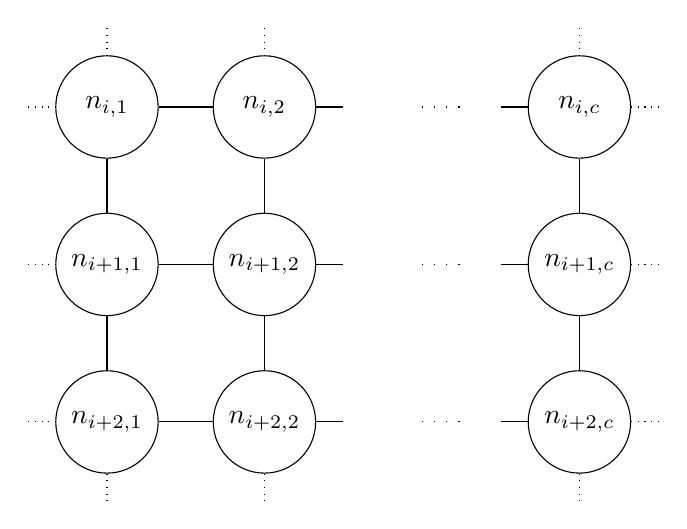
\begin{tikzpicture}[scale=1]
	% Default action for each node
	\tikzstyle{every node}=[draw, shape=circle, minimum size=1.3cm];

	% MIDDLE

										\coordinate (northleft) at (0, 2);		\coordinate (northright) at (2, 2);
	\coordinate (westup) at (-1,1);		\node (r1c1) at (0,1) {$n_{i,1}$};		\node (r1c2) at (2,1) {$n_{i,2}$};		\coordinate (eastup) at (3,1);
	\coordinate (westmid) at (-1,-1);	\node (r2c1) at (0,-1) {$n_{i+1,1}$};	\node (r2c2) at (2,-1) {$n_{i+1,2}$};	\coordinate (eastmid) at (3,-1);
	\coordinate (westdown) at (-1,-3);	\node (r3c1) at (0,-3) {$n_{i+2,1}$};	\node (r3c2) at (2,-3) {$n_{i+2,2}$};	\coordinate (eastdown) at (3,-3);
										\coordinate (southleft) at (0, -4);		\coordinate (southright) at (2, -4);

	% ellipses
	\coordinate (ellipsis westup) at (4,1);		\coordinate (ellipsis eastup) at (4.5,1);
	\coordinate (ellipsis westmid) at (4,-1);	\coordinate (ellipsis eastmid) at (4.5,-1);
	\coordinate (ellipsis westdown) at (4,-3);	\coordinate (ellipsis eastdown) at (4.5,-3);


	% RHS
											\coordinate (rhs north) at (6, 2);
	\coordinate (rhs westup) at (5,1);		\node (r1cn) at (6,1) {$n_{i,c}$};		\coordinate (rhs eastup) at (7,1);
	\coordinate (rhs westmid) at (5,-1);	\node (r2cn) at (6,-1) {$n_{i+1,c}$};	\coordinate (rhs eastmid) at (7,-1);
	\coordinate (rhs westdown) at (5,-3);	\node (r3cn) at (6,-3) {$n_{i+2,c}$};	\coordinate (rhs eastdown) at (7,-3);
											\coordinate (rhs south) at (6, -4);

	% Horizontals
	\draw[outside] (westup) -- (r1c1);
	\draw (r1c1) -- (r1c2);
	\draw (r1c2) -- (eastup);

	\draw[outside] (westmid) -- (r2c1);
	\draw (r2c1) -- (r2c2);
	\draw (r2c2) -- (eastmid);

	\draw[outside] (westdown) -- (r3c1);
	\draw (r3c1) -- (r3c2);
	\draw (r3c2) -- (eastdown);


	\draw[ellipsis] (ellipsis westup) -- (ellipsis eastup);
	\draw[ellipsis] (ellipsis westmid) -- (ellipsis eastmid);
	\draw[ellipsis] (ellipsis westdown) -- (ellipsis eastdown);


	\draw (rhs westup) -- (r1cn);
	\draw[outside] (r1cn) -- (rhs eastup);

	\draw (rhs westmid) -- (r2cn);
	\draw[outside] (r2cn) -- (rhs eastmid);

	\draw (rhs westdown) -- (r3cn);
	\draw[outside] (r3cn) -- (rhs eastdown);

	% Verticals
	\draw[outside] (northleft) -- (r1c1);
	\draw (r1c1) -- (r2c1);
	\draw (r2c1) -- (r3c1);
	\draw[outside] (r3c1) -- (southleft);

	\draw[outside] (northright) -- (r1c2);
	\draw (r1c2) -- (r2c2);
	\draw (r2c2) -- (r3c2);
	\draw[outside] (r3c2) -- (southright);

	\draw[outside] (rhs north) -- (r1cn);
	\draw (r1cn) -- (r2cn);
	\draw (r2cn) -- (r3cn);
	\draw[outside] (r3cn) -- (rhs south);
\end{tikzpicture}



%% Definition B algorithm

\subsection{Algorithm}

\begin{enumerate}
\item Let $n_{i+2,2}$ be the unique vertex in the set $\AdjVV(n_{i+1,2}) \setminus \{ n_{i+1,1} , n_{i+1,3} , n_{i,2} \} $.
\item Let $N = \AdjVV(n_{i+1,1}) \cap \AdjVV(n_{i+2,2})$ be the common neighbours of $n_{i+1,1}$ and $n_{i+2,2}$.
If the number of common neighbours $\card{N}$ is not exactly two, fail the procedure.
\item We know that $n_{i+1,2} \in N$ by construction. Let $n_{i+2,1}$ be the other vertex in $N$.
\item If either of $n_{i+2,1}$ or $n_{i+2,2}$ is in $\Visited$, fail the procedure. Otherwise add the two vertices to $\Visited$.
\item Ensure that the visited neighbours of $n_{i+2,1}$ and $n_{i+2,2}$ are exactly as specified,
that is $n_{i+2,1} \cap \Visited = \{ n_{i+2,2} , n_{i+1,1} \}$ and $n_{i+2,2} \cap \Visited = \{ n_{i+2,1} , n_{i+1,2} \}$.
If this is not the case, remove $n_{i+2,1}$ and $n_{i+2,2}$ from $\Visited$ and fail the procedure.





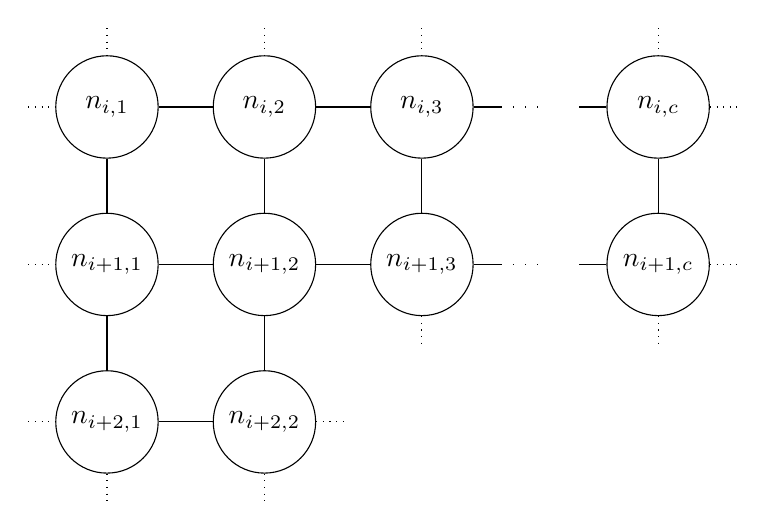
\begin{tikzpicture}[scale=1]
	% Default action for each node
	\tikzstyle{every node}=[draw, shape=circle, minimum size=1.3cm];

	% MIDDLE

										\coordinate (northleft) at (0, 2);		\coordinate (northmid) at (2, 2);		\coordinate (northright) at (4, 2);
	\coordinate (westup) at (-1,1);		\node (r1c1) at (0,1) {$n_{i,1}$};		\node (r1c2) at (2,1) {$n_{i,2}$};		\node (r1c3) at (4,1) {$n_{i,3}$};		\coordinate (eastup) at (5,1);
	\coordinate (westmid) at (-1,-1);	\node (r2c1) at (0,-1) {$n_{i+1,1}$};	\node (r2c2) at (2,-1) {$n_{i+1,2}$};	\node (r2c3) at (4,-1) {$n_{i+1,3}$};	\coordinate (eastmid) at (5,-1);
	\coordinate (westdown) at (-1,-3);	\node (r3c1) at (0,-3) {$n_{i+2,1}$};	\node (r3c2) at (2,-3) {$n_{i+2,2}$};											\coordinate (eastdown) at (3,-3);
										\coordinate (southleft) at (0, -4);		\coordinate (southmid) at (2, -4);		\coordinate (southright) at (4, -2);

	% ellipses
	\coordinate (ellipsis westup) at (5,1);		\coordinate (ellipsis eastup) at (5.5,1);
	\coordinate (ellipsis westdown) at (5,-1);	\coordinate (ellipsis eastdown) at (5.5,-1);


	% RHS
											\coordinate (rhs north) at (7, 2);
	\coordinate (rhs westup) at (6,1);		\node (r1cn) at (7,1) {$n_{i,c}$};		\coordinate (rhs eastup) at (8,1);
	\coordinate (rhs westmid) at (6,-1);	\node (r2cn) at (7,-1) {$n_{i+1,c}$};	\coordinate (rhs eastmid) at (8,-1);
											\coordinate (rhs south) at (7, -2);

	% Horizontals
	\draw[outside] (westup) -- (r1c1);
	\draw (r1c1) -- (r1c2) -- (r1c3) -- (eastup);

	\draw[outside] (westmid) -- (r2c1);
	\draw (r2c1) -- (r2c2) -- (r2c3) -- (eastmid);

	\draw[outside] (westdown) -- (r3c1);
	\draw (r3c1) -- (r3c2);
	\draw[outside] (r3c2) -- (eastdown);


	\draw[ellipsis] (ellipsis westup) -- (ellipsis eastup);
	\draw[ellipsis] (ellipsis westdown) -- (ellipsis eastdown);


	\draw (rhs westup) -- (r1cn);
	\draw[outside] (r1cn) -- (rhs eastup);

	\draw (rhs westmid) -- (r2cn);
	\draw[outside] (r2cn) -- (rhs eastmid);


	% Verticals
	\draw[outside] (northleft) -- (r1c1);
	\draw (r1c1) -- (r2c1);
	\draw (r2c1) -- (r3c1);
	\draw[outside] (r3c1) -- (southleft);

	\draw[outside] (northmid) -- (r1c2);
	\draw (r1c2) -- (r2c2);
	\draw (r2c2) -- (r3c2);
	\draw[outside] (r3c2) -- (southmid);

	\draw[outside] (northright) -- (r1c3);
	\draw (r1c3) -- (r2c3);
	\draw[outside] (r2c3) -- (southright);


	\draw[outside] (rhs north) -- (r1cn);
	\draw (r1cn) -- (r2cn);
	\draw[outside] (r2cn) -- (rhs south);
\end{tikzpicture}




\item For each column\footnote{Possibly none if $c = 3$} $j \in [3..c-1]$:
	\begin{enumerate}
	\item Let $n_{i+2,j}$ be the unique vertex in the set $\AdjVV(n_{i+1,j}) \setminus \{ n_{i+1,j-1} , n_{i+1,j+1} , n_{i,j} \}$.
	\item If $n_{i+2,j} \in \Visited$, remove all vertices in $r_{i+2}$ from $\Visited$, that is $\{ n_{i+2,k} \mid k \in [1..j] \}$ and fail the procedure.
	Otherwise, add $n_{i+2,j}$ $\Visited$.
	\item Ensure that visited neighbours of $n_{i+2,j}$ are exactly $n_{i+2,j-1}$, $n_{i+1,j}$.
	If this is not the case remove vertices $\{ n_{i+2,k} \mid k \in [1..j] \}$ from $\Visited$ and fail the procedure.
	\end{enumerate}




% Foreach j diagram
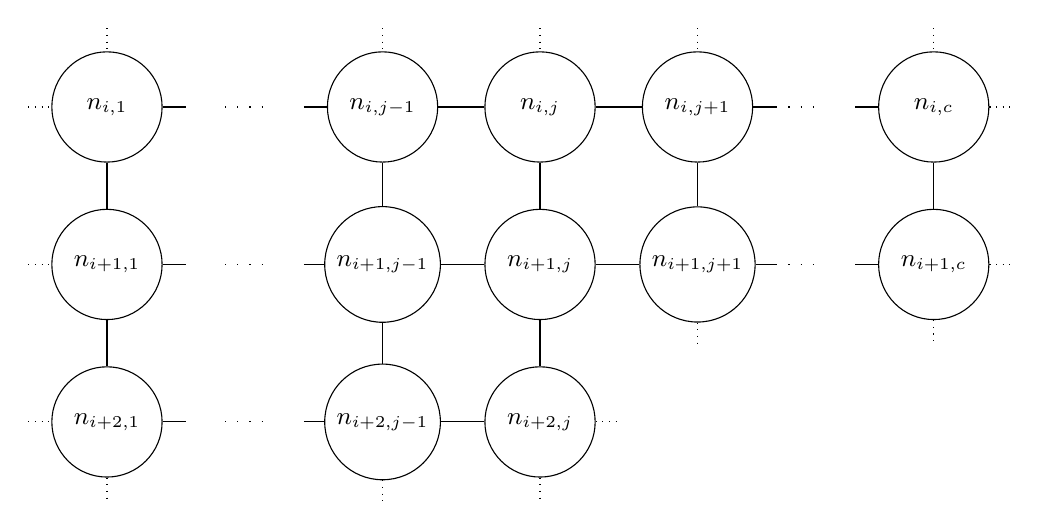
\begin{tikzpicture}[scale=1]
	% Default action for each node
	\tikzstyle{every node}=[draw, shape=circle, minimum size=1.4cm, font=\small];

	% LHS
												\coordinate (lhs north) at (-3.5, 2);
	\coordinate (lhs westup) at (-4.5,1);		\node (r1c0) at (-3.5,1) {$n_{i,1}$};		\coordinate (lhs eastup) at (-2.5,1);
	\coordinate (lhs westmid) at (-4.5,-1);		\node (r2c0) at (-3.5,-1) {$n_{i+1,1}$};	\coordinate (lhs eastmid) at (-2.5,-1);
	\coordinate (lhs westdown) at (-4.5,-3);	\node (r3c0) at (-3.5,-3) {$n_{i+2,1}$};	\coordinate (lhs eastdown) at (-2.5,-3);
												\coordinate (lhs south) at (-3.5, -4);

	% LHS ellipses
	\coordinate (lhs ellipsis westup) at (-2,1);	\coordinate (lhs ellipsis eastup) at (-1.5,1);
	\coordinate (lhs ellipsis westmid) at (-2,-1);	\coordinate (lhs ellipsis eastmid) at (-1.5,-1);
	\coordinate (lhs ellipsis westdown) at (-2,-3);	\coordinate (lhs ellipsis eastdown) at (-1.5,-3);


	% MIDDLE
										\coordinate (northleft) at (0, 2);		\coordinate (northmid) at (2, 2);		\coordinate (northright) at (4, 2);
	\coordinate (westup) at (-1,1);		\node (r1c1) at (0,1) {$n_{i,j-1}$};	\node (r1c2) at (2,1) {$n_{i,j}$};		\node (r1c3) at (4,1) {$n_{i,j+1}$};	\coordinate (eastup) at (5,1);
	\coordinate (westmid) at (-1,-1);	\node (r2c1) at (0,-1) {$n_{i+1,j-1}$};	\node (r2c2) at (2,-1) {$n_{i+1,j}$};	\node (r2c3) at (4,-1) {$n_{i+1,j+1}$};	\coordinate (eastmid) at (5,-1);
	\coordinate (westdown) at (-1,-3);	\node (r3c1) at (0,-3) {$n_{i+2,j-1}$};	\node (r3c2) at (2,-3) {$n_{i+2,j}$};											\coordinate (eastdown) at (3,-3);
										\coordinate (southleft) at (0, -4);		\coordinate (southmid) at (2, -4);		\coordinate (southright) at (4, -2);

	% rhs ellipses
	\coordinate (rhs ellipsis westup) at (5,1);		\coordinate (rhs ellipsis eastup) at (5.5,1);
	\coordinate (rhs ellipsis westdown) at (5,-1);	\coordinate (rhs ellipsis eastdown) at (5.5,-1);


	% RHS
											\coordinate (rhs north) at (7, 2);
	\coordinate (rhs westup) at (6,1);		\node (r1cn) at (7,1) {$n_{i,c}$};		\coordinate (rhs eastup) at (8,1);
	\coordinate (rhs westmid) at (6,-1);	\node (r2cn) at (7,-1) {$n_{i+1,c}$};	\coordinate (rhs eastmid) at (8,-1);
											\coordinate (rhs south) at (7, -2);

	% Horizontals
	\draw[outside] (lhs westup) -- (r1c0);
	\draw (r1c0) -- (lhs eastup);

	\draw[outside] (lhs westmid) -- (r2c0);
	\draw (r2c0) -- (lhs eastmid);

	\draw[outside] (lhs westdown) -- (r3c0);
	\draw (r3c0) -- (lhs eastdown);


	\draw (westup) -- (r1c1) -- (r1c2) -- (r1c3) -- (eastup);

	\draw (westmid) -- (r2c1) -- (r2c2) -- (r2c3) -- (eastmid);

	\draw (westdown) -- (r3c1) -- (r3c2);
	\draw[outside] (r3c2) -- (eastdown);


	\draw[ellipsis] (lhs ellipsis westup) -- (lhs ellipsis eastup);
	\draw[ellipsis] (lhs ellipsis westmid) -- (lhs ellipsis eastmid);
	\draw[ellipsis] (lhs ellipsis westdown) -- (lhs ellipsis eastdown);

	\draw[ellipsis] (rhs ellipsis westup) -- (rhs ellipsis eastup);
	\draw[ellipsis] (rhs ellipsis westdown) -- (rhs ellipsis eastdown);


	\draw (rhs westup) -- (r1cn);
	\draw[outside] (r1cn) -- (rhs eastup);

	\draw (rhs westmid) -- (r2cn);
	\draw[outside] (r2cn) -- (rhs eastmid);


	% Verticals
	\draw[outside] (lhs north) -- (r1c0);
	\draw (r1c0) -- (r2c0) -- (r3c0);
	\draw[outside] (r3c0) -- (lhs south);


	\draw[outside] (northleft) -- (r1c1);
	\draw (r1c1) -- (r2c1) -- (r3c1);
	\draw[outside] (r3c1) -- (southleft);

	\draw[outside] (northmid) -- (r1c2);
	\draw (r1c2) -- (r2c2) -- (r3c2);
	\draw[outside] (r3c2) -- (southmid);

	\draw[outside] (northright) -- (r1c3);
	\draw (r1c3) -- (r2c3);
	\draw[outside] (r2c3) -- (southright);


	\draw[outside] (rhs north) -- (r1cn);
	\draw (r1cn) -- (r2cn);
	\draw[outside] (r2cn) -- (rhs south);
\end{tikzpicture}







\item Consider $\AdjVV(n_{i+2,c-1}) \cap \AdjVV(n_{i+1,c})$, the common neighbours of $n_{i+2,c-1}$ and $n_{i+1,c}$.
If these are not exactly two neighbours, remove vertices $\{ n_{i+2,k} \mid k \in [1..c-1] \}$ from $\Visited$ and fail the procedure.
\item One of the two neighbours must be $n_{i+1,c}$ by construction. Let $n_{i+2,c}$ denote the other neighbour.
\item If $n_{i+2,c} \in \Visited$, remove vertices $\{ n_{i+2,k} \mid k \in [1..c-1] \}$ from $\Visited$ and fail the procedure.
Otherwise, add $n_{i+2,c}$ to $\Visited$.
\item Ensure that the visited neighbours of $n_{i+2,c}$ are exactly $\{ n_{i+2,c-1} , n_{i+1,c} \}$,
that is $\AdjVV(n_{i+2,c}) \cap \Visited = \{ n_{i+2,c-1} , n_{i+1,c} \}$. If this is not the case remove vertices $\{ n_{i+2,k} \mid k \in [1..c] \}$ from $\Visited$ and fail the procedure.




% lastnode diagram
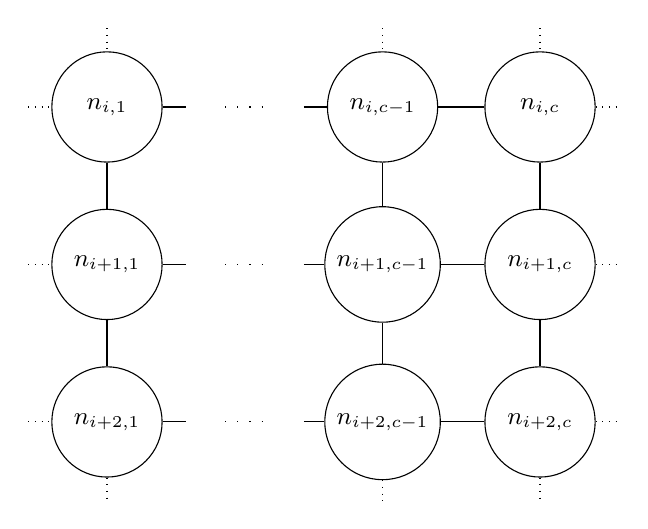
\begin{tikzpicture}[scale=1]
	% Default action for each node
	\tikzstyle{every node}=[draw, shape=circle, minimum size=1.4cm, font=\small];

	% LHS
												\coordinate (lhs north) at (-1.5, 2);
	\coordinate (lhs westup) at (-2.5,1);		\node (r1c0) at (-1.5,1) {$n_{i,1}$};		\coordinate (lhs eastup) at (-0.5,1);
	\coordinate (lhs westmid) at (-2.5,-1);		\node (r2c0) at (-1.5,-1) {$n_{i+1,1}$};	\coordinate (lhs eastmid) at (-0.5,-1);
	\coordinate (lhs westdown) at (-2.5,-3);	\node (r3c0) at (-1.5,-3) {$n_{i+2,1}$};	\coordinate (lhs eastdown) at (-0.5,-3);
												\coordinate (lhs south) at (-1.5, -4);

	% LHS ellipses
	\coordinate (lhs ellipsis westup) at (0,1);		\coordinate (lhs ellipsis eastup) at (0.5,1);
	\coordinate (lhs ellipsis westmid) at (0,-1);	\coordinate (lhs ellipsis eastmid) at (0.5,-1);
	\coordinate (lhs ellipsis westdown) at (0,-3);	\coordinate (lhs ellipsis eastdown) at (0.5,-3);


	% MIDDLE
										\coordinate (northmid) at (2, 2);		\coordinate (northright) at (4, 2);
	\coordinate (westup) at (1,1);		\node (r1c2) at (2,1) {$n_{i,c-1}$};	\node (r1c3) at (4,1) {$n_{i,c}$};		\coordinate (eastup) at (5,1);
	\coordinate (westmid) at (1,-1);	\node (r2c2) at (2,-1) {$n_{i+1,c-1}$};	\node (r2c3) at (4,-1) {$n_{i+1,c}$};	\coordinate (eastmid) at (5,-1);
	\coordinate (westdown) at (1,-3);	\node (r3c2) at (2,-3) {$n_{i+2,c-1}$};	\node (r3c3) at (4,-3) {$n_{i+2,c}$};	\coordinate (eastdown) at (5,-3);
										\coordinate (southmid) at (2, -4);		\coordinate (southright) at (4, -4);




	% Horizontals
	\draw[outside] (lhs westup) -- (r1c0);
	\draw (r1c0) -- (lhs eastup);

	\draw[outside] (lhs westmid) -- (r2c0);
	\draw (r2c0) -- (lhs eastmid);

	\draw[outside] (lhs westdown) -- (r3c0);
	\draw (r3c0) -- (lhs eastdown);


	\draw (westup) -- (r1c2) -- (r1c3);
	\draw[outside] (r1c3) -- (eastup);

	\draw (westmid) -- (r2c2) -- (r2c3);
	\draw[outside] (r2c3) -- (eastmid);

	\draw (westdown) -- (r3c2) -- (r3c3);
	\draw[outside] (r3c3) -- (eastdown);


	\draw[ellipsis] (lhs ellipsis westup) -- (lhs ellipsis eastup);
	\draw[ellipsis] (lhs ellipsis westmid) -- (lhs ellipsis eastmid);
	\draw[ellipsis] (lhs ellipsis westdown) -- (lhs ellipsis eastdown);


	% Verticals
	\draw[outside] (lhs north) -- (r1c0);
	\draw (r1c0) -- (r2c0) -- (r3c0);
	\draw[outside] (r3c0) -- (lhs south);

	\draw[outside] (northmid) -- (r1c2);
	\draw (r1c2) -- (r2c2) -- (r3c2);
	\draw[outside] (r3c2) -- (southmid);

	\draw[outside] (northright) -- (r1c3);
	\draw (r1c3) -- (r2c3) -- (r3c3);
	\draw[outside] (r3c3) -- (southright);

\end{tikzpicture}

\item Return the vertices of node row $r_{i+2}$, that is $n_{i+2,1} \cdots n_{i+2,c}$.
\end{enumerate}





%%%% PHASE 3

\section{Phase 3: Extend rows}
%% Phase 3.1 summary
``Extend a row'' is iteratively applied, starting from $r_1 = n_{1,1} \cdots n_{1,c}$ and $r_2 = n_{2,1} \cdots n_{2,c}$, to yield successive rows until it fails.
The resulting rows are appended \emph{below} $\Structured$.


%% Phase 3.1 diagram
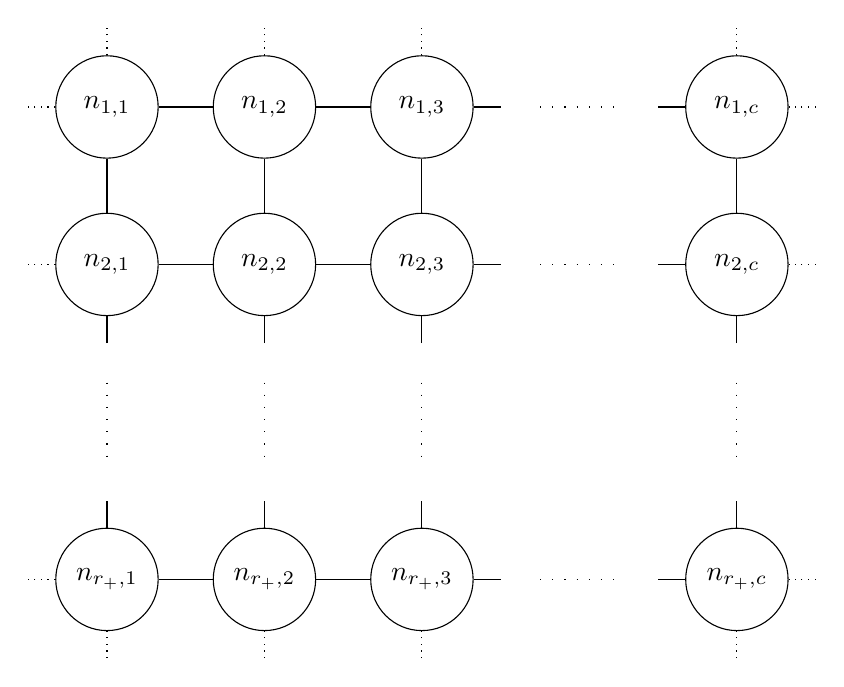
\begin{tikzpicture}
	\tikzstyle{every node}=[draw, shape=circle, minimum size=1.3cm];

	% First rows
	\drawellipsiscol{num=2, rowoffset=6, coloffset=7.5}
	\drawgrid{rows=2, cols=3, rowoffset=6,
		labeler=\plainlabelnode, labelerA=0, labelerB=0,
		southborder=structured, eastborder=structured}
	\drawgrid{rows=2, cols=1, rowoffset=6, coloffset=8,
		labeler=\varcollabelnode, labelerA=0, labelerB=0, labelerC=c,
		southborder=structured, westborder=structured}

	% Bottom horizontal ellipsis
	\drawellipsisrow{num=3, rowoffset=0.5}
	\drawellipsisrow{num=1, rowoffset=0.5, coloffset=8}

	% Last row
	\drawellipsiscol{num=1, rowoffset=0, coloffset=7.5}
	\drawgrid{rows=1, cols=3, rowoffset=0,
		labeler=\varrowlabelnode, labelerA=0, labelerB=0, labelerC=r_+,
		northborder=structured, eastborder=structured}
	\drawgrid{rows=1, cols=1, rowoffset=0, coloffset=8,
		labeler=\varlabelnode, labelerA=0, labelerB=0, labelerC=r_+, labelerD=c,
		northborder=structured, westborder=structured}
\end{tikzpicture}




%% Phase 3.2 summary
``Extend a row'' is iteratively applied, starting from the mirror image of the initial rows about the x-axis, that is $r_1 = n_{2,1} \cdots n_{2,c}$ and $r_2 = n_{1,1} \cdots n_{1,c}$, to yield successive rows until it fails.
The resulting rows are appended \emph{above} $\Structured$.

%% Phase 3.2 diagram
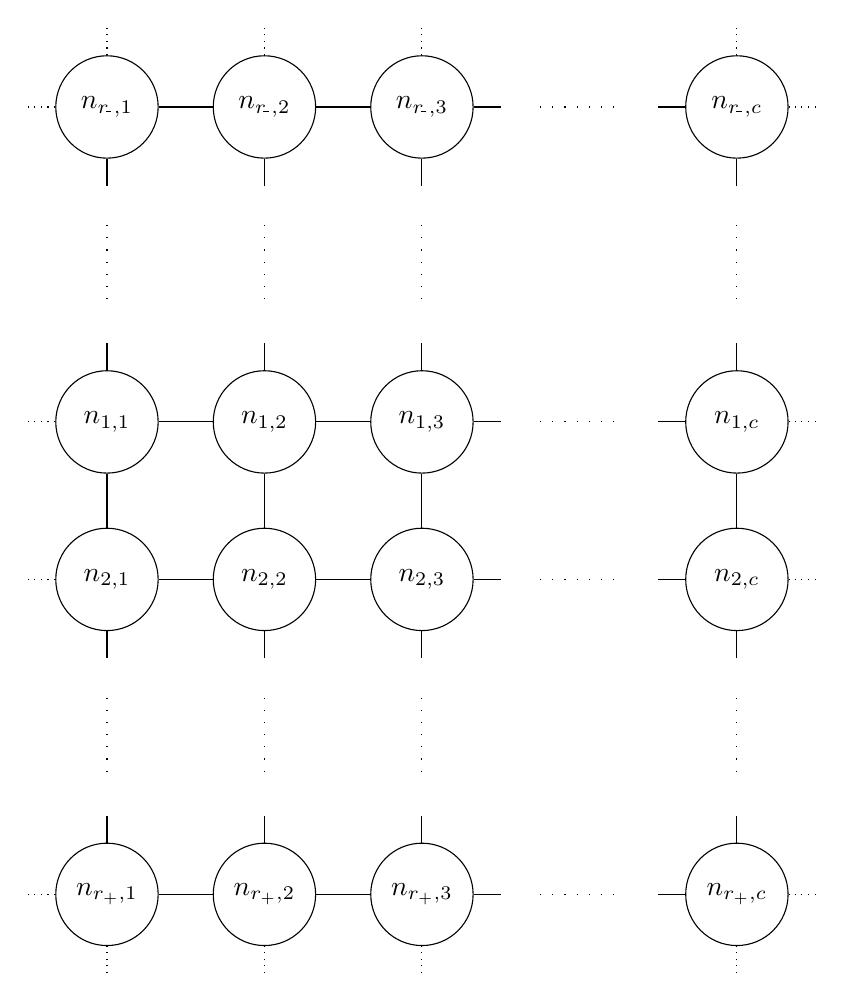
\begin{tikzpicture}
	\tikzstyle{every node}=[draw, shape=circle, minimum size=1.3cm];

	% First first rows
	\drawellipsiscol{num=1, rowoffset=10, coloffset=7.5}
	\drawgrid{rows=1, cols=3, rowoffset=10,
		labeler=\varrowlabelnode, labelerA=0, labelerB=0, labelerC=r_{\!^{\_}},
		southborder=structured, eastborder=structured}
	\drawgrid{rows=1, cols=1, rowoffset=10, coloffset=8,
		labeler=\varlabelnode, labelerA=0, labelerB=0, labelerC=r_{\!^{\_}}, labelerD=c,
		southborder=structured, westborder=structured}

	% Top horizontal ellipsis
	\drawellipsisrow{num=3, rowoffset=6.5}
	\drawellipsisrow{num=1, rowoffset=6.5, coloffset=8}

	% First rows
	\drawellipsiscol{num=2, rowoffset=6, coloffset=7.5}
	\drawgrid{rows=2, cols=3, rowoffset=6,
		labeler=\plainlabelnode, labelerA=0, labelerB=0,
		southborder=structured, eastborder=structured, northborder=structured}
	\drawgrid{rows=2, cols=1, rowoffset=6, coloffset=8,
		labeler=\varcollabelnode, labelerA=0, labelerB=0, labelerC=c,
		southborder=structured, westborder=structured, northborder=structured}

	% Bottom horizontal ellipsis
	\drawellipsisrow{num=3, rowoffset=0.5}
	\drawellipsisrow{num=1, rowoffset=0.5, coloffset=8}

	% Last row
	\drawellipsiscol{num=1, rowoffset=0, coloffset=7.5}
	\drawgrid{rows=1, cols=3, rowoffset=0,
		labeler=\varrowlabelnode, labelerA=0, labelerB=0, labelerC=r_+,
		northborder=structured, eastborder=structured}
	\drawgrid{rows=1, cols=1, rowoffset=0, coloffset=8,
		labeler=\varlabelnode, labelerA=0, labelerB=0, labelerC=r_+, labelerD=c,
		northborder=structured, westborder=structured}
\end{tikzpicture}


%% Phase 3 algorithm

\subsection{Algorithm}

\paragraph{Extend below}
\begin{enumerate}
\item Let $r_a = n_{1,1} \cdots n_{1,c}$ and $r_b = n_{2,1} \cdots n_{2,c}$ be the first two structured node rows.
\item \label{step:extend_row} Let $n_{i,1} \cdots n_{i,c}$ and $n_{i+1,1} \cdots n_{i+1,c}$ represent the respective elements of $r_a$ and $r_b$.
\item Call the procedure ``Extend a row'' with $r_a$ and $r_b$ as inputs.
\item If the procedure fails, go to step~\ref{step:init_reverse_row}.
\item Otherwise, append the new row obtained $r_{new} = n_{i+2,1} \cdots n_{i+2,c}$ \emph{below} $\Structured$.\\
Thus $\Structured$ will become:
$\begin{bmatrix}
	n_{1,1}   & n_{1,2}   & \cdots  & n_{1,c}   \\
	n_{2,1}   & n_{2,2}   & \cdots  & n_{2,c}   \\
	\vdots    & \vdots    &         & \vdots    \\
	n_{i,1}   & n_{i,2}   & \cdots  & n_{i,c}   \\
	n_{i+1,1} & n_{i+1,2} & \cdots  & n_{i+1,c} \\
	n_{i+2,1} & n_{i+2,2} & \cdots  & n_{i+2,c}
	\end{bmatrix}$
\item Set $r_a = n_{i+1,1} \cdots n_{i+1,c}$ and $r_b = n_{i+2,1} \cdots n_{i+2,c}$, and continue from step~\ref{step:extend_row}.
\end{enumerate}

\paragraph{Extend above}
\begin{enumerate}[resume]
\item \label{step:init_reverse_row} Let $r_a = n_{2,1} \cdots n_{2,c}$ and $r_b = n_{1,1} \cdots n_{1,c}$ be the first two structured node rows, the other way around.
\item \label{step:reverse_extend_row} Let $n_{i,1} \cdots n_{i,c}$ and $n_{i+1,1} \cdots n_{i+1,c}$ represent the respective elements of $r_a$ and $r_b$.
\item Call the procedure ``Extend a row'' with $r_a$ and $r_b$ as inputs.
\item If the procedure fails, return immediately.
\item Otherwise, append the new row obtained $r_{new} = n_{i+2,1} \cdots n_{i+2,c}$ \emph{above} $\Structured$.\\
Thus $\Structured$ will become:
$\begin{bmatrix}
	n_{i+2,1} & n_{i+2,2} & \cdots  & n_{i+2,c} \\
	n_{i+1,1} & n_{i+1,2} & \cdots  & n_{i+1,c} \\
	n_{i,1}   & n_{i,2}   & \cdots  & n_{i,c}   \\
	\vdots    & \vdots    &         & \vdots    \\
	n_{1,1}   & n_{1,2}   & \cdots  & n_{1,c}   \\
	n_{2,1}   & n_{2,2}   & \cdots  & n_{2,c}   \\
	\vdots    & \vdots    &         & \vdots    \\
	n_{r_+,1} & n_{r_+,2} & \cdots  & n_{r_+,c}
	\end{bmatrix}$
\item Set $r_a = n_{i+1,1} \cdots n_{i+1,c}$ and $r_b = n_{i+2,1} \cdots n_{i+2,c}$, and continue from step~\ref{step:reverse_extend_row}.
\end{enumerate}

\section{Sketch proof of complexity analysis}
We argue that the length-first search algorithm presented in this chapter runs in $O(\Structured)$, that is linear in the size of the detected structured region\footnote{If no structured region is detected, then we take this to mean that the run-time should be constant, $O(1)$.}.

Neighbour queries are performed using the relation-maps available, and are hence assumed to run in $O(1)$. Set operations such as set-intersection and set-difference between a constant neighbours also run in $O(1)$, as we assume some (again small) constant upper bound on the number of neighbours.

Querying the visited set or adding a vertex to it is done in $O(1)$.

If the algorithm terminates having not found any structure region, which can only occur in the \emph{grow a quad} phase, then it would have only examined a constant number of neighbours and applied a constant number of set-operations.

If the algorithm terminates having found a structured region, then it must have called the ``extend a quad'' and ``extend rows'' functions a number of times linear in $\Structured$. We know this since each call to those functions adds a new vertex to $\Structured$. All other remaining work performed is linear in time.

Thus the time complexity of the length-first search algorithm is $O(\Structured)$.

\subsection{A corollary}
Given that length-first search runs in $O(\Structured)$, we show that using it for detecting multiple structure regions results in an $O(\VertexSet)$ time complexity.

For every application of length-first search, we detect $\Structured$ vertices in $O(\Structured)$ time. Vertices which are detected are added to the visited set and hence are not used as a starting vertex in the future. Since length-first search consumes as many vertices as it consumes time (asymptotically speaking), then by the end we would have exhausted all vertices, and have done so in $O(\VertexSet$).

\section{Chapter summary}
In this chapter we refined our sketch of the length-first search algorithm into a more precise form more amenable for complexity analysis. On this basis we analyse the algorithmic complexity of the algorithm, and find it to be linear in the number of vertices.



\end{document}
